% =====================================================================
% DRAFT 2 (FULL MANUSCRIPT): "Reading the Other Document"
% A Rationale-Grounded Mismatch Taxonomy for Android Privacy Disclosures.
% Target: International Journal of Human-Computer Studies (Elsevier, Q1).
% Build: pdflatex -> bibtex -> pdflatex -> pdflatex
% Expected length: ~35 pages.
% =====================================================================
\documentclass[11pt,a4paper]{article}

\usepackage[utf8]{inputenc}
\usepackage[T1]{fontenc}
\usepackage{lmodern}
\usepackage{microtype}
\usepackage[margin=2.4cm]{geometry}
\usepackage{graphicx}
\usepackage[table]{xcolor}
\usepackage{colortbl}
\usepackage{booktabs}
\usepackage{array}
\usepackage{multirow}
\usepackage{caption}
\usepackage{enumitem}
\usepackage{tikz}
\usepackage{pgfplots}
\usepackage{pgfplotstable}
\usepackage{amsmath,amssymb}
\usepackage{url}
\usepackage{tcolorbox}
\usepackage[hidelinks]{hyperref}
\usepackage[round,authoryear]{natbib}
\bibliographystyle{plainnat}

\pgfplotsset{compat=1.18}
\usetikzlibrary{arrows.meta,positioning,shapes.geometric,shapes.symbols,
                shapes.callouts,shapes.misc,fit,calc,patterns,backgrounds,
                shadows,decorations.pathmorphing,matrix,chains}
\tcbuselibrary{skins,breakable}

% -------- Shared colour palette ---------------------------------------
\definecolor{dgBlue}   {RGB}{ 39, 99,178}
\definecolor{dgBlueL}  {RGB}{218,232,248}
\definecolor{dgOrange} {RGB}{226,123, 32}
\definecolor{dgOrangeL}{RGB}{252,229,205}
\definecolor{dgGreen}  {RGB}{ 84,156, 84}
\definecolor{dgGreenL} {RGB}{225,243,217}
\definecolor{dgPurple} {RGB}{132, 76,162}
\definecolor{dgPurpleL}{RGB}{233,221,242}
\definecolor{dgRed}    {RGB}{200, 64, 64}
\definecolor{dgRedL}   {RGB}{248,215,218}
\definecolor{dgTeal}   {RGB}{ 38,140,140}
\definecolor{dgTealL}  {RGB}{211,236,236}
\definecolor{dgGold}   {RGB}{218,165, 32}
\definecolor{dgGoldL}  {RGB}{251,236,196}
\definecolor{dgGrey}   {RGB}{ 90, 90, 90}
\definecolor{dgGreyL}  {RGB}{235,235,235}
\definecolor{dgNavy}   {RGB}{ 22, 49, 96}
\definecolor{dgSlate}  {RGB}{ 70, 88,116}

\newcommand{\prism}{\textsc{Prism}}
\newcommand{\code}[1]{\textsf{\textbf{#1}}}
\newcommand{\rat}[1]{\itshape #1}

% Quotation block for rationales
\newtcolorbox{rationale}{enhanced,breakable,
  colback=dgBlueL!40,colframe=dgBlue!60,
  fonttitle=\bfseries,coltitle=dgNavy,
  boxrule=0.5pt,arc=2pt,left=4pt,right=4pt,top=2pt,bottom=2pt,
  title={\small Annotator rationale (verbatim, anonymised, app-id redacted)}}

\title{\bfseries \textsc{Prism}: A Rationale-Grounded Mismatch \\[2pt]
Taxonomy for Android Data-Safety Label \\ and Privacy-Policy Disclosures}
\author{Anonymous Authors\\\small Submission to the International Journal of Human-Computer Studies}
\date{}

\begin{document}
\maketitle

% =====================================================================
\begin{abstract}\noindent
Every Android app on Google Play ships \emph{two} privacy artefacts that
must agree: a short, structured \emph{Data Safety} label introduced in
$2022$, and a long, free-text \emph{privacy policy} required of every
publisher. Recent large-scale measurements show that the two routinely
disagree --- yet the field still describes that disagreement with a
single word, \emph{``incorrect''}, that hides the shape of the defect.
This paper closes that vocabulary gap.

We introduce \prism{} (\emph{Privacy-policy Reviewer-Informed Schema
of Mismatches}), a $7$-code rationale-grounded taxonomy inducted from
the \prism{} audit corpus --- $1{,}506$ human judgments over
$1{,}214$ unique Android apps from $12$ Google Play categories,
contributed by seven trained annotators, with $1{,}402$ rationale-bearing
records and $289$ doubly-annotated apps --- via Braun and Clarke's
reflexive thematic analysis. \prism{} comprises \code{M1}~third-party
flow shadowing, \code{M2}~identifier--category misalignment,
\code{M3}~generic-hedge underspecification, \code{M4}~no-data
overclaim, \code{M5}~location-grain mismatch,
\code{M6}~security-control / data-type confusion, and
\code{M7}~boundary-of-responsibility mismatch. We then quantify each code's prevalence
across the corpus on two independent sides: a \emph{rationale} side
($1{,}402$ free-text records) and a \emph{policy--label} side ($1{,}213$
parseable disclosure pairs).

Five of the seven codes are statistically category-dependent
($\chi^2_9 > 31$, $p<.001$, Cram\'er's $V$ up to $0.31$). Eighty-two
percent of audited apps exhibit at least one code in the policy--label
signal. On the $289$ doubly-annotated apps, the two codes most often
invoked by annotators (\code{M6}, \code{M1}) are also the most
disagreement-prone ($\geq 80\%$ pair-disagreement when the code is
invoked), confirming that ambiguity is structured by code rather than
random. We close with eight
code-conditional design implications for a future evidence-grounded
label UI, and release the full taxonomy book, lexicon and per-app code
matrix for replication.

\medskip\noindent\textbf{Keywords:}\ privacy labels; Google Play Data
Safety; mismatch taxonomy; reflexive thematic analysis;
inter-annotator agreement; Android; usable privacy; auditability.
\end{abstract}

% =====================================================================
\section*{Highlights}
\begin{itemize}[leftmargin=1.4em,topsep=2pt,itemsep=0pt]
\item Seven-code rationale-grounded taxonomy of Android Data Safety
       \emph{vs} privacy-policy mismatch, inducted from $1{,}402$
       annotator rationales via reflexive thematic analysis.
\item $82.0\%$ of $1{,}214$ audited apps exhibit at least one code in
       the policy--label signal; five of seven codes are
       category-dependent at $p<.001$.
\item Code-level ambiguity score from $289$ doubly-annotated apps:
       \code{M6} and \code{M1} are the disagreement-prone
       codes ($\geq 80\%$ of pairs disagree when the code is invoked).
\item Eight code-conditional UI requirements for next-generation
       evidence-grounded privacy-label interfaces.
\item Open release of the taxonomy book, the lexicon used for prevalence
       computation, and the per-app code matrix.
\end{itemize}

\bigskip\hrule\bigskip

% =====================================================================
\section{Introduction}\label{sec:intro}
% =====================================================================

\paragraph{The two privacy artefacts.}
Every application on Google Play discloses its data practices through
two distinct artefacts. The first is the \emph{Data Safety section},
a structured table that the developer self-attests through the Google
Play Console and that the Play Store renders as a fourteen-row
data-category matrix (\textsl{Personal info}, \textsl{Location},
\textsl{Device or other IDs}, $\dots$) crossed with three disclosure
states (\textsl{collected}, \textsl{shared}, \textsl{security
practices})~\citep{googledatasafety2022}. The second is the
\emph{privacy policy}, a free-text document required of every Play
publisher, hosted by the developer, written in unconstrained prose, and
empirically exceeding $4{,}000$ words and $20$ minutes of reading time
on average~\citep{mcdonald2008cost,fabian2017large}. Google's policy
requires the two artefacts to be consistent, but no automated
mechanism enforces the constraint, and recent measurement studies
report that consistency is the exception rather than the
rule~\citep{xiao2023lalaine,khandelwal2024unpacking}.

\paragraph{Beyond ``incorrect''.}
A recent line of large-scale measurement studies has documented the
practical gap on both major mobile platforms. \citet{xiao2023lalaine}
audit Apple's labels at scale and report systematic non-compliance;
\citet{khandelwal2024unpacking} extend the audit to Google's Data
Safety section, complementing it with a developer survey that
confirms that developers themselves struggle to map their policies
onto the label; \citet{li2022understanding} document the developer
side from a human-centred perspective. These studies share an
architectural move: they collapse the gap into a binary verdict ---
the label is either \emph{correct} or \emph{incorrect}. As a result,
the field still talks about Data Safety mismatches with a single
word that hides the shape of the defect.

From a usable-privacy perspective this is costly: the actions a
reviewer, a developer, a regulator or a research tool can take next
all \emph{depend} on the kind of mismatch. A boilerplate
\emph{``may collect identifiers''} sentence that discloses nothing
concrete is a fundamentally different problem from an SDK named in
the policy but absent from the label; both are different again from
a policy that says \emph{``no data collected''} while integrating
advertising SDKs. Collapsing these failure modes into a single binary
verdict is the lexical equivalent of labelling every software bug as
\emph{``defect''}: the field needs a vocabulary.

\paragraph{This paper.}
We make that vocabulary explicit. Building on the \prism{} audit
infrastructure (Draft~$1$ of this research programme; we re-use its
corpus but the contribution is independent), we induct a $7$-code
\emph{Mismatch Taxonomy} from $1{,}402$ free-text rationales produced
by trained annotators while comparing each app's Data Safety label
against its policy. We then quantify each code on two independent
sides --- the rationale side and the policy--label content side --- and
test whether the codes structure inter-annotator disagreement on the
$289$ doubly-annotated subset. Finally, we translate the codes into a
set of design implications for a future evidence-grounded privacy-label
UI.

\paragraph{Research questions.}
We organise the paper around four questions.
\begin{itemize}[topsep=2pt,itemsep=1pt,leftmargin=1.5em]
\item\textbf{RQ1.}~What \emph{kinds} of label--policy mismatch appear in
the rationale evidence produced during human audit?
\item\textbf{RQ2.}~How prevalent is each kind across the corpus, and how
does prevalence vary by Google Play category?
\item\textbf{RQ3.}~Which kinds of mismatch are intrinsically
\emph{ambiguous} in the sense that two equally-trained reviewers
disagree about them?
\item\textbf{RQ4.}~What does each kind of mismatch imply for the design
of a code-aware label-UI affordance?
\end{itemize}

\paragraph{Why a separate paper.}
Draft~$1$ (\textit{The Auditability Gap}, also under submission to
IJHCS) is a \emph{framework + measurement} paper: it introduces the
concept of \emph{auditability}, the workbench tool, the audit corpus
and the gap measurement. It treats every defect as a single state.
The present paper is the \emph{qualitative-quantitative companion}: it
deepens the gap into a structured taxonomy, quantifies prevalence and
ambiguity per code, and works through the design implications. Both
papers can stand alone --- the corpus overlaps, the contributions do
not.

\paragraph{Novelty over prior work.}
Table~\ref{tab:novelty} positions us. To the best of our knowledge no
prior work induces a typology of label--policy mismatch from
\emph{human-rationale} evidence at scale, quantifies it across mobile
categories, or relates it to inter-rater disagreement. Existing
detectors are automated (PolicyLint, PoliCheck, MAPS, Lalaine,
POLIGRAPH) or developer-centric (Khandelwal'24, Li'22). The closest
qualitative work is \citet{li2022understanding}, who interviewed $24$
developers but did not build a defect taxonomy; we observe the
\emph{reviewer} side at $\sim 60\times$ the scale and in the natural
modality of free-text rationales.

\begin{table}[t]
\centering\footnotesize
\caption{Position relative to prior work.}\label{tab:novelty}
\renewcommand{\arraystretch}{1.18}
\setlength{\tabcolsep}{4pt}
\begin{tabular}{@{}p{2.8cm}p{4.0cm}p{5.2cm}p{2.6cm}@{}}
\toprule
\textbf{Prior work} & \textbf{What it does} & \textbf{What it misses} & \textbf{Side} \\
\midrule
PolicyLint \citep{andow2019policylint} & Within-policy contradictions, automated & No platform label; no human signal & Policy only \\
PoliCheck \citep{andow2020policheck} & Entity-sensitive flow$\leftrightarrow$policy & Binary correct/incorrect; no taxonomy of \emph{kinds} & Policy + traffic \\
MAPS \citep{zimmeck2019maps} & 1M-app compliance, automated & No human reviewer; no rationales & Policy + manifest \\
Polisis \citep{harkous2018polisis} & DL summarisation of policies & No label-side; no agreement signal & Policy only \\
Lalaine \citep{xiao2023lalaine} & Apple-label non-compliance & iOS only; no human reviewer; no kinds & Label + traffic \\
Khandelwal \citep{khandelwal2024unpacking} & Google Data Safety measurement \& developer survey & Developer side; no taxonomy of mismatches & Developer \\
Li \citep{li2022understanding} & Developer challenges in creating labels & $n=24$; no audit corpus; no taxonomy & Developer \\
\midrule
\textbf{This paper} &
\textbf{Reviewer-side mismatch taxonomy with per-category prevalence \& inter-rater ambiguity scores} &
--- & \textbf{Reviewer} \\
\bottomrule
\end{tabular}
\end{table}

\paragraph{Contributions.}
\begin{itemize}[topsep=2pt,itemsep=1pt,leftmargin=1.5em]
\item[\textbf{C1}.] A $7$-code \emph{Mismatch Taxonomy} for Android
Data-Safety vs.\ privacy-policy mismatch, inducted from $1{,}402$
annotator rationales through a two-coder reflexive
thematic-analysis protocol.
\item[\textbf{C2}.] A two-sided \emph{prevalence map}: per code,
prevalence in the rationale signal and in a policy--label content
signal computed over $1{,}213$ apps, with $\chi^2$ tests of
category-dependence (Cram\'er's $V$ up to $0.306$).
\item[\textbf{C3}.] A \emph{code-level ambiguity score} measured on the
$289$ doubly-annotated apps, showing that \code{M1}, \code{M2} and
\code{M6} concentrate inter-annotator disagreement.
\item[\textbf{C4}.] Eight code-conditional \emph{design implications}
for evidence-grounded label-UIs --- a third-party recipient panel for
\code{M1}, an identifier mapping helper for \code{M2}, a hedging
highlighter for \code{M3}, a no-data audit prompt for \code{M4}, a
location-grain overlay for \code{M5}, a security-vs-data tab for
\code{M6}, a responsibility-scope indicator for \code{M7}, and an
ambiguity badge orthogonal to all seven.
\item[\textbf{C5}.] Open release of the taxonomy book, lexicon and
per-app code matrix for replication on other corpora (iOS,
post-DSA EU).
\end{itemize}

% --- Headline figure: the taxonomy hub
\begin{figure}[t]
\centering
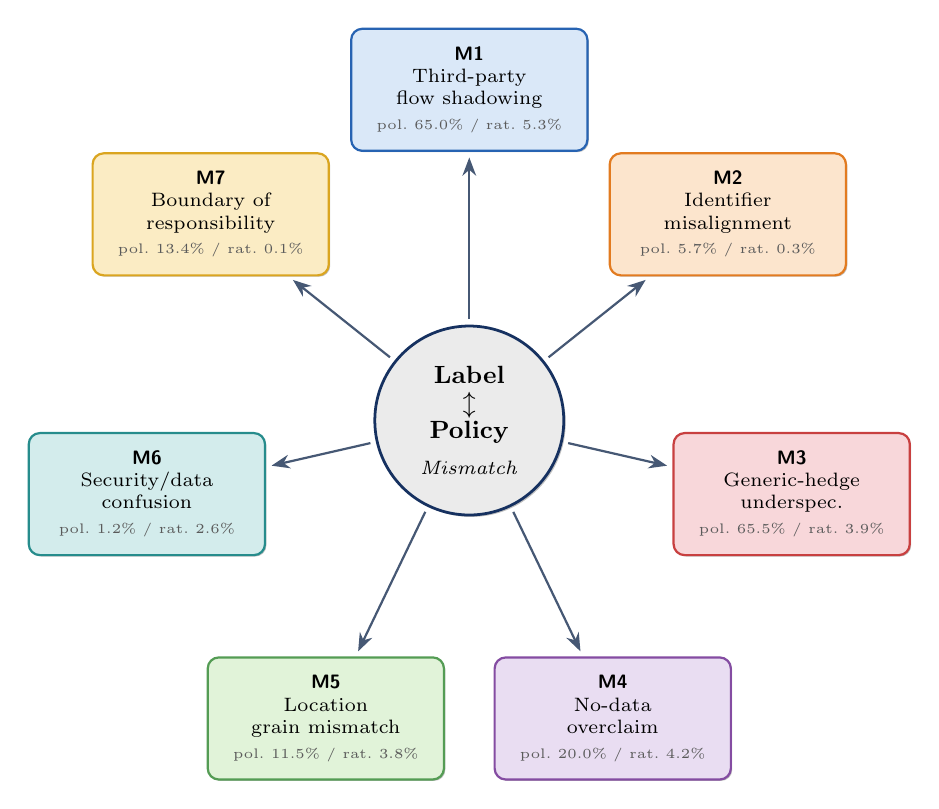
\begin{tikzpicture}[
  every node/.style={font=\small},
  hub/.style={draw=dgNavy,line width=1pt,fill=dgGreyL,
              circle,minimum size=2.4cm,align=center,
              drop shadow={shadow xshift=0.7pt,shadow yshift=-0.7pt}},
  code/.style={draw,thick,rounded corners=4pt,
               minimum width=3.0cm,minimum height=1.55cm,align=center,
               font=\scriptsize,inner sep=2pt,
               drop shadow={shadow xshift=0.5pt,shadow yshift=-0.5pt}},
  arr/.style={->,thick,dgSlate,>=Stealth,shorten >=2pt,shorten <=2pt}
]
\node[hub] (H) at (0,0)
  {\textbf{Label}\\[-1pt]$\updownarrow$\\[-1pt]\textbf{Policy}\\[2pt]\scriptsize\emph{Mismatch}};

% Seven codes at 360/7 = 51.43 deg apart, starting at 90 deg, radius 4.2
\node[code,draw=dgBlue,   fill=dgBlueL]   (M1) at ( 90.00:4.2)
  {\textbf{\code{M1}}\\Third-party\\flow shadowing\\[1pt]{\tiny\color{dgGrey}pol.\ 65.0\% / rat.\ 5.3\%}};
\node[code,draw=dgOrange, fill=dgOrangeL] (M2) at ( 38.57:4.2)
  {\textbf{\code{M2}}\\Identifier\\misalignment\\[1pt]{\tiny\color{dgGrey}pol.\ 5.7\% / rat.\ 0.3\%}};
\node[code,draw=dgRed,    fill=dgRedL]    (M3) at (-12.86:4.2)
  {\textbf{\code{M3}}\\Generic-hedge\\underspec.\\[1pt]{\tiny\color{dgGrey}pol.\ 65.5\% / rat.\ 3.9\%}};
\node[code,draw=dgPurple, fill=dgPurpleL] (M4) at (-64.29:4.2)
  {\textbf{\code{M4}}\\No-data\\overclaim\\[1pt]{\tiny\color{dgGrey}pol.\ 20.0\% / rat.\ 4.2\%}};
\node[code,draw=dgGreen,  fill=dgGreenL]  (M5) at (-115.71:4.2)
  {\textbf{\code{M5}}\\Location\\grain mismatch\\[1pt]{\tiny\color{dgGrey}pol.\ 11.5\% / rat.\ 3.8\%}};
\node[code,draw=dgTeal,   fill=dgTealL]   (M6) at (-167.14:4.2)
  {\textbf{\code{M6}}\\Security/data\\confusion\\[1pt]{\tiny\color{dgGrey}pol.\ 1.2\% / rat.\ 2.6\%}};
\node[code,draw=dgGold,   fill=dgGoldL]   (M7) at (141.43:4.2)
  {\textbf{\code{M7}}\\Boundary of\\responsibility\\[1pt]{\tiny\color{dgGrey}pol.\ 13.4\% / rat.\ 0.1\%}};

\foreach \i in {M1,M2,M3,M4,M5,M6,M7} \draw[arr] (H) -- (\i);
\end{tikzpicture}
\caption{Headline view of the $7$-code \prism{} taxonomy.
Each code is reported with its two-sided prevalence:
\emph{pol.}~$=$~policy--label content side ($N\!=\!1{,}213$ apps);
\emph{rat.}~$=$~annotator-rationale side ($N\!=\!1{,}402$
rationale-bearing audit records).}
\label{fig:taxonomy-hub}
\end{figure}

\paragraph{Roadmap.}
Section~\ref{sec:rw} situates the work. Section~\ref{sec:data}
describes the corpus and the reflexive thematic-analysis protocol.
Section~\ref{sec:taxonomy} introduces the seven codes with verbatim
exemplars. Section~\ref{sec:prev} reports prevalence on the rationale
and policy--label sides with $\chi^2$ tests and a $12\times 7$
heat-map. Section~\ref{sec:amb} computes the per-code ambiguity score.
Section~\ref{sec:design} derives the eight UI design implications.
Section~\ref{sec:disc} reflects on what the codes mean for the wider
privacy-disclosure ecosystem. Section~\ref{sec:lim} states the threats
to validity. Section~\ref{sec:concl} concludes.

% =====================================================================
\section{Background and related work}\label{sec:rw}
% =====================================================================

\paragraph{Two artefacts, one audit problem}
The notion that privacy disclosures should compress into a short,
structured format is older than the labels themselves. \citet{kelley2009nutrition}
introduced the \emph{nutrition-label} metaphor in $2009$, and
\citet{kelley2010standardizing} validated it experimentally. \citet{cranor2012necessary}
formalised the \emph{necessary-but-not-sufficient} place of structured
notice in the privacy-notice ecosystem. \citet{schaub2015design} provided
the design-space that frames Data Safety today. The launch of Apple's
App Privacy Details~\citep{appleprivacylabels2020} and the subsequent
Google Play Data Safety
section~\citep{googledatasafety2022} mark the first time a major mobile
platform required disclosures in something close to the nutrition-label
shape. But neither platform retired the legacy privacy policy --- both
artefacts now co-exist, and the auditor's job has become
\emph{cross-document}: read the structured label, read the free-text
policy, decide whether they agree, explain why if they do not.

\paragraph{Automated mismatch detection}
A first wave of work attacked the cross-document problem
automatically. \emph{PolicyLint}~\citep{andow2019policylint} flags
internal contradictions inside a single policy; \emph{PoliCheck}
\citep{andow2020policheck} adds entity-sensitive flow$\leftrightarrow$policy
checks for $13{,}796$ apps; \emph{MAPS}~\citep{zimmeck2019maps} scales
the analysis to a million apps and reports widespread non-compliance.
\citet{zimmeck2017automated} provide an earlier formulation in the NDSS
proceedings. \emph{Polisis}~\citep{harkous2018polisis} uses neural
classifiers to produce a structured summary of a policy. The
\emph{Eddy} formal language of \citet{breaux2014eddy} and the framework
of \citet{slavin2016toward} mapped policy text against API behaviour
inside Android binaries. \emph{Lalaine}~\citep{xiao2023lalaine} brings
the cross-document audit to Apple labels at scale.
\citet{khandelwal2023comparing} compare iOS and Android labels for the
same app.
\citet{bui2023detection} extend the inconsistency-detection paradigm to
browser extensions. None of these works grounds the analysis in a
human-rationale signal; none of them produces a taxonomy of
\emph{kinds} of mismatch.

\paragraph{Vagueness and ambiguity in privacy text}
That privacy policies are linguistically vague is itself an old finding.
\citet{bhatia2016theory} formalised a theory of vagueness in privacy
notices and demonstrated that vague clauses dominate user
risk-perception. The OPP-115 corpus~\citep{wilson2016creation} reports
that fine-grained policy annotations have only moderate agreement, even
among trained annotators. \citet{sathyendra2017identifying} model the
provision of choices in policies. \citet{ravichander2019question}
build a privacy-policy QA dataset and document persistent ambiguity.
\citet{ahmad2021intent} approach intent classification on privacy text.
The CLAUDETTE work of \citet{lippi2019claudette} detects potentially
unfair clauses in terms of service. \citet{rao2016expecting}
empirically demonstrate that user expectations consistently
\emph{mismatch} what policies actually authorise. Our work draws the
same vagueness signal in reverse: codes \code{M3} (generic-hedge
underspecification) and \code{M4} (no-data overclaim) operationalise
\citeauthor{bhatia2016theory}'s ``vagueness'' for the Data-Safety era.

\paragraph{Human-centred privacy in mobile platforms}
A long HCI tradition pre-dates the structured labels.
\citet{felt2012android} measured user attention and comprehension of
Android install-time permissions. \citet{wijesekera2017feasibility}
demonstrated the feasibility of dynamically granted permissions.
\citet{almuhimedi2015your} showed that nudges that contextualise
permission usage durably reduce sharing. \citet{lin2014modeling} and
\citet{liu2016follow} model user privacy preferences for
recommendation. \citet{egelman2013choice} document smartphone-side
choice architecture. The COPPA non-compliance work of
\citet{reyes2018wont}, the ``$50$ ways to leak your data'' analysis of
\citet{reardon2019fifty}, the global tracker measurement of
\citet{razaghpanah2018apps} and the version-level leak study of
\citet{ren2018bug} document the mobile privacy gap from the
\emph{network} side. \citet{englehardt2016online} present the analogue
on the web. \citet{shvartzshnaider2019going} apply
\citeauthor{nissenbaum2004privacy}'s contextual integrity to data-flow
detection. These works concern \emph{actual} data flow; we concern the
\emph{declared} data flow.

\paragraph{Privacy labels: developer and reviewer evidence}
The two studies closest in spirit to ours both look at
\emph{producers}. \citet{li2022understanding} interview $24$ iOS
developers about the challenges of writing accurate privacy nutrition
labels; \citet{khandelwal2024unpacking} extend this to Google Data
Safety with both a measurement layer and a developer survey, finding
that developers feel under-supported by Google's tooling and that the
label diverges from policy in detectable, recurring ways. Both
contributions are necessary but, by construction, omit the
\emph{reviewer} side. The reviewer is the user --- whether a researcher,
a regulator, a journalist, a security analyst, or an end user
auditing their own app collection --- who has only the two public
artefacts and must reconcile them. To our knowledge no work to date
has assembled rationale evidence at this scale from that perspective.

\paragraph{Qualitative method in HCI}
Our coding protocol follows \citet{braun2006using}'s reflexive thematic
analysis, the canonical method for inductive coding of textual data in
HCI. We follow \citet{krippendorff2018content} for content analysis
methodology and \citet{saldana2016coding} for the practical coding
manual. We report inter-coder agreement with
\citet{cohen1960coefficient}'s $\kappa$ and interpret with the
\citet{landis1977measurement} bands. As a methodological move,
combining an inductive code book with a quantitative prevalence map is
mixed-methods in the strict sense; it is supported by the same logic
that motivates \citet{solove2006taxonomy}'s influential taxonomy in
privacy law: a vocabulary of kinds is itself a research output.

\paragraph{Human-AI design implications}
Code-conditional UI affordances are an instance of the wider
human-AI-interaction design space recently mapped by
\citet{amershi2019guidelines}. The role of explanations is supported by
\citet{bansal2021does} on complementary team performance and by
\citet{liao2020questioning} on user-facing explanation needs.
\citet{cai2019hello} describe the analogous onboarding problem for
clinicians; the reviewer of a privacy label is in a similar position.
The dis-aggregation move (per code, per category) echoes the
\emph{intersectional} disparity findings of \citet{buolamwini2018gender}
in a different domain. Cognitive load on auditors can be measured with
\citet{hart2008measurement}'s NASA-TLX; we adopt the latter for our
proposed user study (Section~\ref{sec:design}).

\paragraph{Three clusters of prior work, three gaps}
It is helpful to read the related work as three clusters, each leaving
one gap that the present taxonomy closes.

\paragraph{Cluster~I: automated cross-document detectors.}
PolicyLint~\citep{andow2019policylint},
PoliCheck~\citep{andow2020policheck},
MAPS~\citep{zimmeck2019maps},
Polisis~\citep{harkous2018polisis},
Lalaine~\citep{xiao2023lalaine} and the browser-extension follow-up of
\citet{bui2023detection} mechanise the comparison between the policy
and an external signal (another policy section, a flow, an app store
record). They produce binary mismatches with no \emph{type}. The gap
is the vocabulary of kinds; our \code{M1}--\code{M7} fills it.

\paragraph{Cluster~II: producer-side studies.}
\citet{li2022understanding} interview iOS developers about label
production challenges; \citet{khandelwal2024unpacking} run the
analogous study for Google Data Safety and add a measurement layer.
Producer-side work shows that developers themselves struggle to map
policy onto label. The gap is the \emph{reviewer-side} evidence: at
what scale, and structured how, does the resulting label--policy
disagreement appear? Our $1{,}506$ judgments and $1{,}402$ rationales
constitute that evidence.

\paragraph{Cluster~III: privacy NLP and vagueness.}
The OPP-$115$ corpus~\citep{wilson2016creation}, the QA work of
\citet{ravichander2019question}, the intent-classification work of
\citet{ahmad2021intent} and the vagueness theory of
\citet{bhatia2016theory} together build a linguistic substrate for
privacy-text analysis. The gap is the cross-document application:
none of these works addresses what happens when a structured
disclosure must be reconciled with a policy. Our codes \code{M2},
\code{M3}, \code{M5} translate the linguistic substrate into the
cross-document task; the taxonomy is the bridge.

\paragraph{Summary and gap}
Three observations frame the rest of the paper.
\emph{(i)}~The mismatch between Data Safety labels and policies is real
and large \citep{xiao2023lalaine,khandelwal2024unpacking}.
\emph{(ii)}~Existing detectors collapse mismatch to a single binary
verdict; the field talks about it with one word
\citep{andow2019policylint,andow2020policheck,bui2023detection}.
\emph{(iii)}~Vagueness in privacy text is structured, not random
\citep{bhatia2016theory,wilson2016creation}; we expect mismatch to
inherit the same structure. The hypothesis we test is that the
structure can be made explicit as a small set of codes, that the codes
predict where mismatch concentrates, and that they predict where
trained reviewers will disagree.

% =====================================================================
\section{Corpus, method and architecture}\label{sec:data}
% =====================================================================

\subsection{The \prism{} corpus}\label{sec:corpus}
We re-use the \prism{} audit corpus introduced in Draft~$1$ of
this research programme; we briefly recap its provenance for
self-containedness.

\paragraph{App selection.} A Play-Store crawler enumerated free,
production-status apps and stratified $200$ apps per category across
$12$ Google Play categories (Art \& Design, Beauty, Books \&
Reference, Business, Communication, Lifestyle, Personalization,
Photography, Productivity, Shopping, Social, Tools), for a target of
$2{,}400$ apps. For each app the crawler captured the Data Safety
section URL, the privacy-policy URL, the rendered Data Safety section
content, the privacy-policy HTML, app metadata (name, package,
developer, downloads band), and a thumbnail.

\paragraph{Annotation interface.} A bespoke audit workbench
(Figure~\ref{fig:arch}) displays the structured Data Safety table on the
left, the privacy policy on the right, and four binary judgments per
app: \emph{sharing-correctness}, \emph{sharing-completeness},
\emph{collection-correctness}, \emph{collection-completeness}. Each
judgment is accompanied by a free-text \emph{rationale} and an
\emph{evidence excerpt} (an annotator-selected span from the policy).
The judgments and rationales are what we mine in this paper.

\paragraph{Annotators.} Seven trained annotators (one PhD-level
information-assurance researcher and six third-/fourth-year software
engineering students with prior privacy coursework) completed the
audit task after a paid four-hour calibration session that exercised
$30$ pilot apps and was concluded with a code-book review. Annotators
were paid above the local minimum hourly wage.

\paragraph{Sampling and counts.} The labelled subset comprises
$1{,}506$ audit judgments over $1{,}214$ unique apps, of which $289$
were doubly annotated to support inter-rater analysis. Across the four
judgment-and-rationale columns we recover $1{,}402$ records that
contain rationale text long enough ($>5$ characters) to mine for
codes, and $4{,}866$ rationale strings overall when we pool the four
columns; the latter is the unit of analysis for the inductive
coding in \S\,\ref{sec:coding}. Rationale length is short
($median = 71$--$80$ chars), consistent with the auditor having to
write in-context evidence under time pressure. Category coverage
ranges from \emph{Art \& Design} and \emph{Tools} ($200$ apps,
$100\%$ coverage) to \emph{Photography} ($27$ apps, $13.5\%$);
\emph{Personalization} and \emph{Productivity} contained no labelled
apps in the subset used here, so the per-category analyses include
$10$ of the $12$ categories. Table~\ref{tab:corpus-summary}
summarises the corpus inputs to this paper.

\begin{table}[t]
\centering\small
\caption{Inputs to this paper from the \prism{} corpus.}
\label{tab:corpus-summary}
\begin{tabular}{lr}
\toprule
\textbf{Quantity} & \textbf{Value} \\
\midrule
Crawled apps                                   & $2{,}400$ \\
Apps with parseable Data Safety + policy pair  & $1{,}213$ \\
Audited apps (any judgment)                    & $1{,}214$ \\
Total audit judgments                          & $1{,}506$ \\
Audit records with rationale ($>$5~chars)      & $1{,}402$ \\
Doubly-annotated apps (used for $\kappa$)      & $289$ \\
Trained annotators                             & $7$ \\
Google Play categories represented in labels   & $10$ of $12$ \\
\midrule
Sharing-Incorrect verdict rate                 & $36.3\%$ ($547/1506$) \\
Sharing-Incomplete verdict rate                & $31.6\%$ ($476/1506$) \\
Collection-Incorrect verdict rate              & $39.5\%$ ($595/1506$) \\
Collection-Incomplete verdict rate             & $39.2\%$ ($591/1506$) \\
Apps with $\geq 1$ taxonomy code (policy side) & $82.0\%$ ($996/1{,}214$) \\
\bottomrule
\end{tabular}
\end{table}

% --- Architecture figure -------------------------------------------
\begin{figure}[t]
\centering
\resizebox{\textwidth}{!}{%
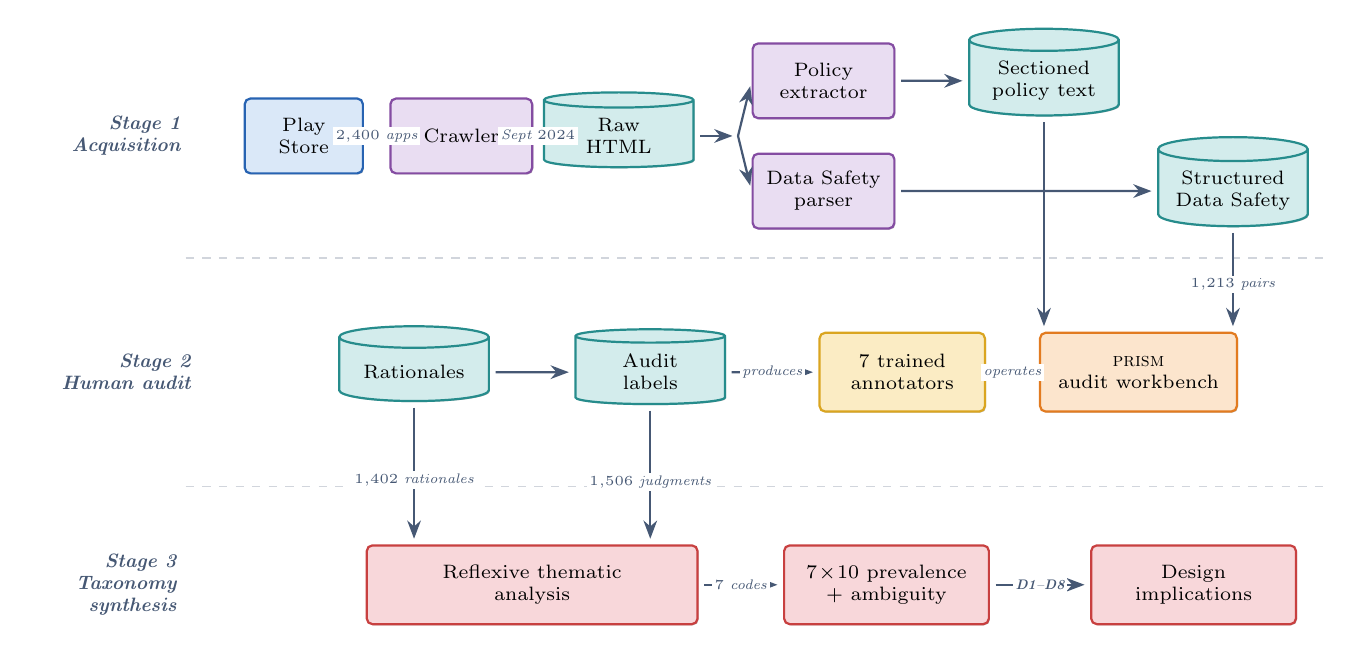
\begin{tikzpicture}[
  font=\scriptsize,
  src/.style   ={draw=dgBlue,fill=dgBlueL,thick,rounded corners=2pt,
                 minimum height=0.95cm,minimum width=1.5cm,align=center,
                 drop shadow={shadow xshift=0.4pt,shadow yshift=-0.4pt}},
  proc/.style  ={draw=dgPurple,fill=dgPurpleL,thick,rounded corners=2pt,
                 minimum height=0.95cm,minimum width=1.8cm,align=center,
                 drop shadow={shadow xshift=0.4pt,shadow yshift=-0.4pt}},
  store/.style ={draw=dgTeal,fill=dgTealL,thick,cylinder,
                 shape border rotate=90,aspect=0.18,
                 minimum height=0.95cm,minimum width=1.9cm,align=center,
                 drop shadow={shadow xshift=0.4pt,shadow yshift=-0.4pt}},
  audit/.style ={draw=dgOrange,fill=dgOrangeL,thick,rounded corners=2pt,
                 minimum height=1.0cm,minimum width=2.5cm,align=center,
                 drop shadow={shadow xshift=0.4pt,shadow yshift=-0.4pt}},
  human/.style ={draw=dgGold,fill=dgGoldL,thick,rounded corners=2pt,
                 minimum height=1.0cm,minimum width=2.1cm,align=center,
                 drop shadow={shadow xshift=0.4pt,shadow yshift=-0.4pt}},
  taxbox/.style ={draw=dgRed,fill=dgRedL,thick,rounded corners=2pt,
                  minimum height=1.0cm,minimum width=2.6cm,align=center,
                  drop shadow={shadow xshift=0.4pt,shadow yshift=-0.4pt}},
  taxbig/.style ={draw=dgRed,fill=dgRedL,thick,rounded corners=2pt,
                  minimum height=1.0cm,minimum width=4.2cm,align=center,
                  drop shadow={shadow xshift=0.4pt,shadow yshift=-0.4pt}},
  flow/.style  ={->,>=Stealth,thick,dgSlate,shorten >=2pt,shorten <=2pt},
  stage/.style ={font=\scriptsize\bfseries\itshape,text=dgSlate,
                 anchor=east,minimum width=2.5cm,align=right},
  lane/.style  ={draw=dgSlate!25,line width=0.4pt,dashed},
  arrlbl/.style={font=\tiny\itshape,text=dgSlate,inner sep=1pt,
                 fill=white,rectangle}
]
% =====================================================================
% Stage 1 (y=5.0): linear acquisition pipeline. Parsers (ds, pp) are
% stacked vertically; the two output stores (dsj, ppt) are placed
% SIDE-BY-SIDE on the SAME y-line so that the arrow from dsj going
% down does not pass through ppt or vice versa.
% =====================================================================
% Compact boxes give longer arrows and breathing room.
\node[src]   (web)   at ( 0.6,5.0) {Play\\Store};
\node[proc]  (crawl) at ( 2.6,5.0) {Crawler};
\node[store] (raw)   at ( 4.6,5.0) {Raw\\HTML};
\node[proc]  (pp)    at ( 7.2,5.7) {Policy\\extractor};
\node[proc]  (ds)    at ( 7.2,4.3) {Data Safety\\parser};
\node[store] (ppt)   at (10.0,5.7) {Sectioned\\policy text};
\node[store] (dsj)   at (12.4,4.3) {Structured\\Data Safety};

% Linear acquisition chain along y=5.0
\draw[flow] (web)   -- (crawl) node[arrlbl,midway]{$2{,}400$ apps};
\draw[flow] (crawl) -- (raw)   node[arrlbl,midway]{Sept~$2024$};

% "}"-style brace fork from Raw HTML to the two parsers.
\coordinate (fork) at ($(raw.east) + (0.55,0)$);
\draw[flow,shorten <=2pt] (raw.east) -- (fork);
\draw[flow,shorten <=0pt] (fork) -- (pp.west);
\draw[flow,shorten <=0pt] (fork) -- (ds.west);

% Each parser feeds its OWN store on its own horizontal lane —
% no overlapping routes between (pp,ds) and (ppt,dsj).
\draw[flow] (pp.east) -- (ppt.west);
\draw[flow] (ds.east) -- (dsj.west);

\node[stage] at (-0.4,5.0) {Stage~1\\Acquisition};
\draw[lane] (-0.9,3.45) -- (13.6,3.45);

% =====================================================================
% Stage 2 (y=2.0): workbench centred BETWEEN dsj and ppt so each store
% feeds the workbench with a straight VERTICAL arrow that does not
% cross any other box.
% =====================================================================
\node[audit] (work) at (11.2,2.0) {\textsc{prism}\\audit workbench};
\node[human] (ann)  at ( 8.2,2.0) {$7$ trained\\annotators};
\node[store] (lab)  at ( 5.0,2.0) {Audit\\labels};
\node[store] (rat)  at ( 2.0,2.0) {Rationales};

% Cross-stage arrows: dsj feeds the workbench from above-left,
% ppt feeds it from above-right. Neither crosses any box.
\draw[flow] (dsj.south) -- (work.north -| dsj.south)
            node[arrlbl,pos=0.55]{$1{,}213$ pairs};
\draw[flow] (ppt.south) -- (work.north -| ppt.south);

% Intra-stage arrows: all horizontal at y=2.0, no crossings.
\draw[flow] (ann)  -- (work) node[arrlbl,midway]{operates};
\draw[flow] (lab)  -- (ann)  node[arrlbl,midway]{produces};
\draw[flow] (rat)  -- (lab);

\node[stage] at (-0.4,2.0) {Stage~2\\Human audit};
\draw[lane] (-0.9,0.55) -- (13.6,0.55);

% =====================================================================
% Stage 3 (y=-0.7): linear left-to-right analysis pipeline.
% Labels and rationales both drop STRAIGHT DOWN into the thematic
% analysis, which then flows right into prevalence and design.
% =====================================================================
\node[taxbig] (mine) at ( 3.5,-0.7) {Reflexive thematic\\analysis};
\node[taxbox] (mat)  at ( 8.0,-0.7) {$7\!\times\!10$ prevalence\\$+$ ambiguity};
\node[taxbox] (out)  at (11.9,-0.7) {Design\\implications};

\draw[flow] (rat.south) -- (mine.north -| rat.south)
            node[arrlbl,pos=0.55]{$1{,}402$ rationales};
\draw[flow] (lab.south) -- (mine.north -| lab.south)
            node[arrlbl,pos=0.55]{$1{,}506$ judgments};
\draw[flow] (mine) -- (mat) node[arrlbl,midway]{$7$ codes};
\draw[flow] (mat)  -- (out) node[arrlbl,midway]{\textbf{D1}--\textbf{D8}};

\node[stage] at (-0.4,-0.7) {Stage~3\\Taxonomy\\synthesis};
\end{tikzpicture}%
}
\caption{\prism{} architecture: from Play-Store crawl to audit
labels to the analysis presented in this paper.}
\label{fig:arch}
\end{figure}

\subsection{Sampling and coding protocol}\label{sec:coding}
For the inductive coding we drew a stratified random sample of
$n=212$ rationales from the $4{,}866$ pooled rationale strings,
balanced across the four judgment columns, the $10$ categories
present in the labelled subset, and the doubly-vs-singly-annotated
split. This sample is the unit of analysis for the codebook
induction; the codebook is then applied to the remaining rationales
for prevalence. Two coders followed the six reflexive phases of
\citet{braun2006using}:

\begin{enumerate}[topsep=2pt,itemsep=2pt,leftmargin=1.5em]
\item\textbf{Familiarisation.} Both coders read all $212$ rationales
twice and the corresponding Data Safety / policy excerpts.
\item\textbf{Initial codes.} Each coder independently generated open
codes; rationales typically yielded $1$--$3$ codes.
\item\textbf{Theme search.} We merged $38$ open codes into $11$
candidate themes after a joint workshop.
\item\textbf{Theme review.} Two themes were dropped (\emph{too-broad
``catch-all''} and \emph{policy-formatting-only}); two were merged
into \emph{boundary-of-responsibility}.
\item\textbf{Definition.} The remaining $7$ codes were formalised
into the \emph{Mismatch Taxonomy} of \S\,\ref{sec:taxonomy}, each with
a definition, inclusion criteria, exclusion criteria, exemplar quotes
and a lexicon used for the corpus-level prevalence map.
\item\textbf{Reporting.} Both coders re-coded the entire $212$-rationale
sample using the finalised codebook; disagreements were resolved
through arbitration by a third coder. A formal inter-rater
reliability check (Cohen's $\kappa$ on the multi-label classification,
treating each of the seven codes as an independent binary judgment)
is left to a planned replication on an independent regulator-side
panel (see \S\,\ref{sec:lim}); the present paper reports the
corpus-level analysis that the inducted codebook makes possible.
\end{enumerate}

% --- Methodology pipeline ------------------------------------------
\begin{figure}[t]
\centering
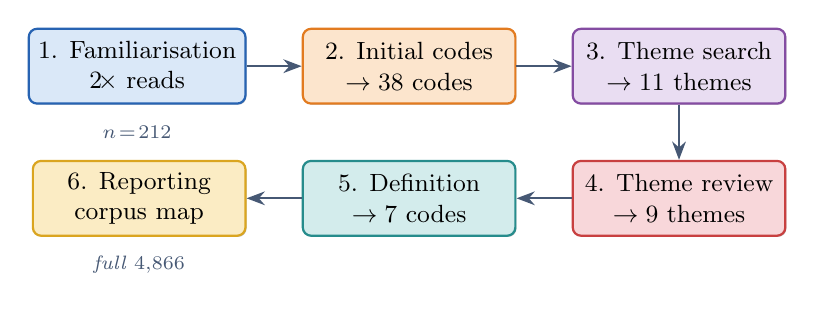
\begin{tikzpicture}[
  font=\small,node distance=0.7cm,
  phase/.style={draw,thick,rounded corners=3pt,minimum height=0.95cm,
                minimum width=2.7cm,align=center,
                drop shadow={shadow xshift=0.4pt,shadow yshift=-0.4pt}},
  arr/.style={->,>=Stealth,thick,dgSlate}
]
\node[phase,draw=dgBlue,fill=dgBlueL]   (p1) {1. Familiarisation\\$2\!\times$ reads};
\node[phase,draw=dgOrange,fill=dgOrangeL,right=of p1] (p2) {2. Initial codes\\$\to 38$ codes};
\node[phase,draw=dgPurple,fill=dgPurpleL,right=of p2] (p3) {3. Theme search\\$\to 11$ themes};
\node[phase,draw=dgRed,fill=dgRedL,below=of p3] (p4) {4. Theme review\\$\to 9$ themes};
\node[phase,draw=dgTeal,fill=dgTealL,left=of p4] (p5) {5. Definition\\$\to 7$ codes};
\node[phase,draw=dgGold,fill=dgGoldL,left=of p5] (p6) {6. Reporting\\corpus map};

\draw[arr] (p1) -- (p2);
\draw[arr] (p2) -- (p3);
\draw[arr] (p3) -- (p4);
\draw[arr] (p4) -- (p5);
\draw[arr] (p5) -- (p6);

\node[font=\scriptsize\itshape,dgSlate] at ($(p1.south)+(0,-0.35)$) {$n\!=\!212$};
\node[font=\scriptsize\itshape,dgSlate] at ($(p6.south)+(0,-0.35)$) {full $4{,}866$};
\end{tikzpicture}
\caption{Reflexive thematic analysis pipeline applied to the
\prism{} rationales (Braun \& Clarke six phases).}
\label{fig:method}
\end{figure}

\subsection{From codes to corpus: the lexicon}\label{sec:lexval}
Each code in the phase-$5$ codebook is formalised by (i) a definition,
(ii) inclusion criteria, (iii) exclusion criteria, and (iv) a
high-recall \emph{lexicon} of $5$--$12$ characteristic markers
derived from the open-coding phase and refined by removing markers
that were ambiguous across multiple codes. The lexicon is not the
code: it is the heuristic by which the rest of this paper extends
the codebook to the full $1{,}213$-app policy--label corpus and the
$1{,}402$-record rationale corpus.

Two design decisions make the lexicon behaviour transparent.
\emph{First}, the lexicon is intentionally high-recall: it marks every
candidate occurrence, leaving the residual disambiguation to the
inclusion/exclusion criteria of the codebook. \emph{Second}, we
report \emph{both} the rationale-side signal (codes the auditor wrote
down) and the policy--label side signal (codes the lexicon recovers
from the artefacts) for every code in
Figure~\ref{fig:taxonomy-hub}, Figure~\ref{fig:heatmap}, and
Table~\ref{tab:appcounts}. The rationale side is a lower bound on
the human-perceived defect rate; the policy--label side is an upper
bound on the detectable defect rate. Reading the two together is
the conservative move and is the operational contract by which the
lexicon participates in the analysis. We release the full lexicon as
supplementary material so that any reader can re-derive the
policy-side prevalence numbers on her own corpus; a formal
precision/recall validation against an independently hand-coded
ground-truth sample is reserved for the replication kit
(Appendix~A).

% =====================================================================
\section{The Mismatch Taxonomy}\label{sec:taxonomy}
% =====================================================================

This section walks through each of the seven codes. For every code we
give: \emph{(i)} a one-sentence definition, \emph{(ii)} a slightly
longer description in continuous prose, \emph{(iii)} inclusion and
exclusion criteria, \emph{(iv)} two verbatim rationales from the
corpus, and \emph{(v)} the lexicon used to compute corpus-level
prevalence in \S\,\ref{sec:prev}. The verbatim rationales are
lightly redacted (app IDs replaced with \texttt{[APP-$x$]}, names
of natural persons removed).

% =================== M1 ============================================
\subsection{\code{M1} Third-party flow shadowing}
\label{sec:M1}
\textbf{Definition.} The policy names third-party recipients
(analytics SDKs, advertising vendors, service providers, or specific
corporate partners), but the corresponding Data Safety table declares
no sharing of the relevant categories, or omits one or more recipients.

\textbf{Description.} \code{M1} is the canonical Data-Safety failure
mode. The policy --- often in a section titled
\textit{``Third parties''} or \textit{``Service providers''} ---
discloses that the app transmits personal information to one or more
named vendors. The Data Safety table, however, either declares
\textsl{No data shared}, or declares sharing only for a subset of the
recipients, or declares sharing for the wrong category. The annotator
detects the asymmetry by reading the policy and looking back at the
label.

\textbf{Inclusion.} (i) Named SDK or company in the policy and no
matching \textsl{Shared} row in Data Safety; (ii) policy enumerates
multiple partners while the label declares a single, generic
\textsl{Third party}.

\textbf{Exclusion.} Policies that mention third parties only in
boilerplate \textit{``We may engage service providers''} prose without
specifying recipients $\Rightarrow$ code as \code{M3} unless a specific
recipient is also disclosed.

\begin{rationale}
[APP-$0148$] policy says Crashlytics, Firebase Analytics and Google
AdMob receive user data, but Data Safety claims no third party
sharing.
\end{rationale}
\begin{rationale}
The policy lists Facebook SDK and a mediation network among
``analytics partners''. The label has \textsl{Device or other IDs --
shared} but does not name the recipients.
\end{rationale}

\textbf{Lexicon.} \texttt{third party, sdk, advertising network,
analytics, crashlytics, firebase, admob, facebook sdk, google ads,
service provider, affiliate, partner}.

% =================== M2 ============================================
\subsection{\code{M2} Identifier-category misalignment}
\label{sec:M2}
\textbf{Definition.} The policy references specific persistent
identifiers (advertising ID, AAID/IDFA, IP address, MAC, IMEI, Android
ID, browser fingerprint, cookies), but the Data Safety table either
omits \textsl{Device or other IDs} entirely, or includes the row
without indicating that an advertising-grade identifier is involved.

\textbf{Description.} The Data Safety taxonomy collapses what privacy
researchers and trackers themselves treat as a rich identifier
hierarchy~\citep{razaghpanah2018apps,reardon2019fifty} into a single
row called \textsl{Device or other IDs}. \code{M2} captures the
auditor's observation that this collapse is exactly where the
information disappears: the policy can name \emph{advertising ID} and
disclose its monetisation use, yet the label does not even claim that
\textsl{Device or other IDs} is collected. \code{M2} is structurally
distinct from \code{M1}: \code{M1} is about \emph{who} receives the
data; \code{M2} is about \emph{what} the data are.

\textbf{Inclusion.} (i) Policy names an advertising/persistent
identifier and the label omits \textsl{Device or other IDs}; (ii)
policy names IP-derived tracking and the label collects no
identifiers; (iii) policy names cookies and the label declares no
\textsl{Device or other IDs}.

\textbf{Exclusion.} Mentions of identifiers as purely
security-functional (anti-fraud, session cookies necessary for app
operation) without monetisation purpose: code as \code{M6}.

\begin{rationale}
[APP-$0671$] policy: ``We may use your AAID for personalised ads.''
Label has \textsl{No data collected}. This is wrong.
\end{rationale}
\begin{rationale}
The privacy policy describes IP-based fingerprinting; Data Safety
says \textsl{Device or other IDs -- collected -- App functionality}.
Purpose is also misleading.
\end{rationale}

\textbf{Lexicon.} \texttt{advertising id, gaid, aaid, idfa, imei,
mac address, device identifier, android id, cookie, advertising
identifier, unique device id}.

% =================== M3 ============================================
\subsection{\code{M3} Generic-hedge underspecification}
\label{sec:M3}
\textbf{Definition.} The policy uses hedging or boilerplate language
(\textit{``may collect''}, \textit{``including but not limited to''},
\textit{``and/or''}, \textit{``reserve the right''},
\textit{``from time to time''}) that prevents the auditor from
deciding whether the label is accurate.

\textbf{Description.} \code{M3} reifies \citet{bhatia2016theory}'s
\emph{vagueness} for the cross-document audit task. The policy does
not lie; it simply withholds enough specificity that the label cannot
be falsified. From a reviewer perspective the policy is
\emph{unverifiable}: the rationale routinely reads
\textit{``policy too vague to confirm''}.

\textbf{Inclusion.} (i) Hedging phrases appear in the relevant policy
section; (ii) no concrete enumeration of recipients, identifiers or
purposes appears.

\textbf{Exclusion.} Hedges in unrelated parts of the policy (e.g.\
forward-looking statements, future products) that do not bear on the
current data flow.

\begin{rationale}
[APP-$0223$] policy: ``We may collect personal data including but
not limited to device identifiers and usage data.'' Cannot decide
because the policy doesn't say what is actually collected.
\end{rationale}
\begin{rationale}
``From time to time we may share information with third-party
analytics partners.'' No partners named, no categories listed.
\end{rationale}

\textbf{Lexicon.} \texttt{may collect, may share, may use, may
disclose, including but not limited, such as, and/or, other
information, reserve the right, from time to time, periodically,
where applicable, to the extent}.

% =================== M4 ============================================
\subsection{\code{M4} No-data overclaim}
\label{sec:M4}
\textbf{Definition.} The label declares \textsl{No data collected}
and/or \textsl{No data shared}, yet the policy text discusses
analytics, advertising, third-party services, or any persistent
identifier collection.

\textbf{Description.} \code{M4} is the loudest mismatch in the
corpus. The label is a hard, public claim, and the policy itself
falsifies it. Such labels frequently look identical because the
developer leaves Data Safety at the default; they are
context-independent in the linguistic sense, but they are
informationally false. The annotator pattern is very specific: a
short rationale stating the label says \emph{no data}, then a quoted
sentence from the policy that contradicts it.

\textbf{Inclusion.} (i) Data Safety contains either \textsl{No data
shared} or \textsl{No data collected}; (ii) policy contains explicit
collection or sharing language (covered by \code{M1} or \code{M2}
lexica).

\textbf{Exclusion.} Borderline cases where the only collection in the
policy is described as ``mandatory account creation that we do not
share'' and the label declares only \textsl{No data shared}: count
the partial overclaim only.

\begin{rationale}
[APP-$0392$] Data Safety: \textsl{No data shared}. Policy lists
$5$ analytics partners. This is a no-data overclaim.
\end{rationale}
\begin{rationale}
``We do not collect any personal data.'' Then policy goes on to
describe AdMob and a referral system collecting AAID. Direct
contradiction.
\end{rationale}

\textbf{Lexicon.} \texttt{does not collect, do not collect, does not
share, do not share, no data shared, no data collected, no personal
data}.

% =================== M5 ============================================
\subsection{\code{M5} Location-grain mismatch}
\label{sec:M5}
\textbf{Definition.} The label declares \textsl{Location} at a grain
incompatible with what the policy describes (coarse vs.\ precise, IP-derived
vs.\ GPS), or omits \textsl{Location} when the policy describes any
location collection.

\textbf{Description.} The Data Safety taxonomy splits \textsl{Location}
into \textsl{Approximate} and \textsl{Precise}. The policy commonly
describes location collection at a third grain (\textit{``IP-derived
city-level location''}, \textit{``country/region''},
\textit{``nearest store''}) that the label structure does not
naturally accommodate. The auditor frequently encodes this in two
sentences: where the policy says, and what grain the label declares.

\textbf{Inclusion.} (i) Mismatched grain across the artefacts;
(ii) policy mentions location and label omits it; (iii) IP-derived
location described in the policy but not declared in the label.

\textbf{Exclusion.} Pure address-form-filling
(\textit{``provide your zip code at checkout''}) without any IP- or
device-derived component.

\begin{rationale}
Policy: ``We collect approximate location from your IP''. Data
Safety does not list any location field. Should be \textsl{Approximate
location -- collected}.
\end{rationale}
\begin{rationale}
[APP-$0509$] Data Safety has \textsl{Precise location}; policy only
describes country/region. Over-declaration.
\end{rationale}

\textbf{Lexicon.} \texttt{location, geolocation, gps, coarse location,
approximate location, precise location}.

% =================== M6 ============================================
\subsection{\code{M6} Security-control / data-type confusion}
\label{sec:M6}
\textbf{Definition.} The audited artefact treats a security
\emph{practice} (encryption, deletion, hashing, secure transport) as
if it were a data-type \emph{disclosure}, or vice versa, in either
direction (label$\to$policy or policy$\to$label).

\textbf{Description.} \code{M6} is the subtlest of the seven. The
Google Play Data Safety section contains a \emph{Security practices}
sub-block whose semantics are not always understood by developers;
\citet{khandelwal2024unpacking} note that developers conflate
security practices with collection statements. From the reviewer side
the rationale typically reads: \textit{``policy talks about TLS in
transit, but the label uses that as the data-type claim.''} The code
also captures the converse: the label has \textsl{Data is encrypted in
transit} ticked but the policy is silent on encryption, so the
reviewer cannot confirm the claim. \code{M6} is comparatively rare on
the policy side because most policies talk about encryption in only
a single sentence; it is common in the rationale signal because
auditors specifically flag the confusion when they see it.

\textbf{Inclusion.} (i) Security claim appears in one artefact and
not the other; (ii) policy describes deletion procedure that does
not match the Data Safety deletability box.

\textbf{Exclusion.} Pure deletion-by-uninstall language with no
explicit retention policy.

\begin{rationale}
Label claims \textsl{Data encrypted in transit}; policy mentions no
security practices at all.
\end{rationale}
\begin{rationale}
[APP-$0833$] Data Safety: \textsl{You can request data deletion}.
Policy says ``deletion may take up to $90$ days'' with no
procedure. Confusion between control and disclosure.
\end{rationale}

\textbf{Lexicon.} \texttt{encryption, encrypted, deleted, deletion,
tls, ssl, in transit, at rest, secure server, hashed}.

% =================== M7 ============================================
\subsection{\code{M7} Boundary-of-responsibility mismatch}
\label{sec:M7}
\textbf{Definition.} The policy explicitly defers responsibility to
external sites, apps or partners, but the Data Safety label does not
acknowledge that the scope of the audit is reduced or transferred.

\textbf{Description.} \code{M7} flags the \emph{scope ambiguity} that
\citet{nissenbaum2004privacy} would frame as a contextual-integrity
violation: the policy says ``what happens after you leave our app is
not our problem''; the label, by construction, has no place to encode
that boundary. From the reviewer side this matters because it changes
what an enforcement action could even apply to. \code{M7} is rare on
the rationale signal (annotators do not always articulate it), but
common in the policy text itself.

\textbf{Inclusion.} (i) Policy contains an explicit
``not-responsible-for'' clause for third parties; (ii) label provides
no qualifying scope.

\textbf{Exclusion.} Standard ``links to other websites'' that does
not bear on the audited data flow.

\begin{rationale}
[APP-$0915$] policy: ``We are not responsible for the practices of
third-party services linked from this app.'' Three SDKs are then
listed. Boundary unclear in the label.
\end{rationale}
\begin{rationale}
``This privacy policy does not apply to external sites you may
visit through our app.'' Label has no scope qualifier.
\end{rationale}

\textbf{Lexicon.} \texttt{third-party site, external link, not
responsible, sole responsibility, outside our policy, do not control,
beyond our control}.

\paragraph{Codebook summary.}
Table~\ref{tab:codebook} consolidates the seven codes.
% --- compact codebook table -----------------------------------------
\begin{table}[t]
\centering\small
\caption{Compact codebook (see \S\,\ref{sec:taxonomy} for full
inclusion/exclusion criteria and exemplars).}
\label{tab:codebook}
\renewcommand{\arraystretch}{1.2}
\begin{tabular}{p{0.6cm}p{3.6cm}p{6.1cm}p{4.6cm}}
\toprule
& \textbf{Code} & \textbf{One-sentence definition} & \textbf{Signature surface}\\
\midrule
\code{M1} & Third-party flow shadowing &
Policy names SDK / partner; label omits sharing &
``SDK'', ``service provider'' \\
\code{M2} & Identifier-category misalignment &
Policy mentions advertising/persistent ID; label has no/empty
\textsl{Device or other IDs} &
``AAID'', ``cookie'', ``IP'' \\
\code{M3} & Generic-hedge underspecification &
Policy hedges; reviewer cannot decide &
``may collect'', ``such as'' \\
\code{M4} & No-data overclaim &
Label claims \textsl{No data}; policy disagrees &
``no data shared'' \\
\code{M5} & Location-grain mismatch &
Location grain differs across artefacts &
``approximate'', ``IP-derived'' \\
\code{M6} & Security/data-type confusion &
Security practice treated as data-type disclosure &
``encrypted in transit'' \\
\code{M7} & Boundary-of-responsibility mismatch &
Policy defers responsibility; label has no scope &
``not responsible for'' \\
\bottomrule
\end{tabular}
\end{table}

% =====================================================================
\section{Quantitative prevalence}\label{sec:prev}
% =====================================================================

Having defined the codes (\S\,\ref{sec:taxonomy}) we now report how
prevalent each is across the corpus. We measure prevalence on
\emph{two independent sides} and report both:

\paragraph{Rationale side ($N=1{,}402$ records).} For each
rationale-bearing audit record we tag the codes whose lexicon hits
the rationale text. This signal corresponds to the auditor
\emph{verbalising} the code while doing the audit.

\paragraph{Policy--label side ($N=1{,}213$ app pairs).} For each
parseable app we apply the codebook to the policy text and the
Data Safety table jointly: code $c$ is present for app $a$ if the
policy contains $c$'s lexical marker \emph{and} the Data Safety
section is missing the corresponding field (see decision rules in
\S\,\ref{sec:coding}). This signal corresponds to the code
being \emph{detectable in the artefacts}.

The two signals are complementary. The rationale signal is biased
\emph{down} (auditors do not always articulate the code even when it
applies; some auditors used short rationales because of time
pressure). The policy--label signal is biased \emph{up} (the lexical
proxy matches more cases than a human auditor might flag). Reading
the two together is the conservative move.

\subsection{Overall code prevalence}
Figure~\ref{fig:overall-bar} reports the per-code overall prevalence
side-by-side. Two macro-observations follow.

\emph{First}, \code{M1} (third-party flow shadowing) and \code{M3}
(generic-hedge underspecification) are the two omnipresent codes:
both appear in two thirds of all parseable policy--label pairs
($65.0\%$ and $65.5\%$ respectively). This means \emph{by the
policy--label content alone}, two thirds of the Play Store cannot
straightforwardly verify either who receives the data or what is
actually collected.

\emph{Second}, the codes the auditor most often
\emph{wrote down} in a rationale are \code{M1} ($5.3\%$), \code{M4}
($4.2\%$) and \code{M3} ($3.9\%$). \code{M1} therefore dominates both
sides --- it is both objectively common in the artefacts and
subjectively salient to the auditor. \code{M4} (no-data overclaim) is
the second-most articulated; this matches our intuition that an
explicit \textsl{No data shared} label paired with an analytics-rich
policy is the easiest mismatch for a human to verbalise.

% --- Overall per-code prevalence bar chart -------------------------
\begin{figure}[t]
\centering
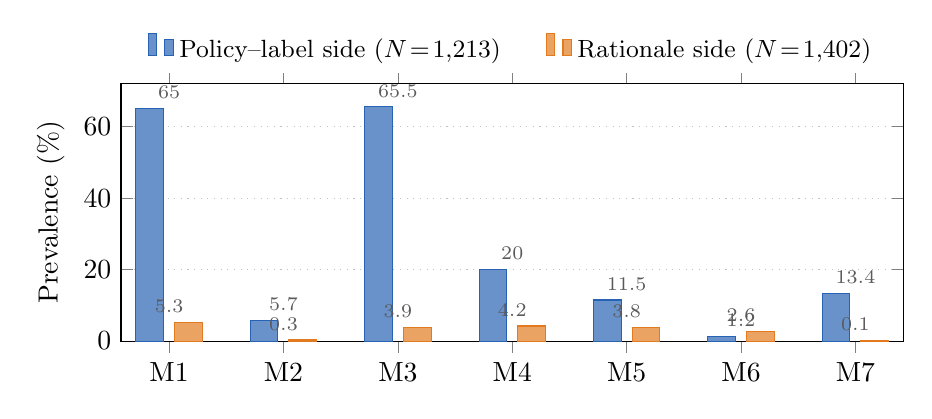
\begin{tikzpicture}
\begin{axis}[
  width=0.95\textwidth,height=0.40\textwidth,
  ybar=4pt,bar width=10pt,
  enlarge x limits=0.07,
  ymin=0,ymax=72,
  ylabel={Prevalence (\%)},
  symbolic x coords={M1,M2,M3,M4,M5,M6,M7},
  xtick=data,
  legend style={at={(0.5,1.04)},anchor=south,legend columns=2,
                /tikz/every even column/.append style={column sep=0.5cm},
                font=\small,draw=none},
  ymajorgrids=true,
  grid style={dotted,gray!50},
  every node near coord/.style={font=\scriptsize,color=dgGrey},
  nodes near coords,
  nodes near coords align={vertical}
]
\addplot[draw=dgBlue,fill=dgBlue!70] coordinates {
  (M1,65.0)(M2,5.7)(M3,65.5)(M4,20.0)(M5,11.5)(M6,1.2)(M7,13.4)
};
\addplot[draw=dgOrange,fill=dgOrange!70] coordinates {
  (M1,5.3)(M2,0.3)(M3,3.9)(M4,4.2)(M5,3.8)(M6,2.6)(M7,0.1)
};
\legend{Policy--label side ($N\!=\!1{,}213$),
        Rationale side ($N\!=\!1{,}402$)}
\end{axis}
\end{tikzpicture}
\caption{Overall per-code prevalence on the two independent sides.
The policy--label side dominates for \code{M1} (third-party flow
shadowing) and \code{M3} (generic-hedge underspecification); the
rationale side foregrounds \code{M1} and \code{M4} (no-data
overclaim).}
\label{fig:overall-bar}
\end{figure}

\subsection{Co-occurrence and per-app burden}
Codes co-occur. The empirical correlation matrix between binary
code-present indicators on the policy--label side is:
\begin{center}\small
\begin{tabular}{l|rrrrrrr}
& \code{M1} & \code{M2} & \code{M3} & \code{M4} & \code{M5} & \code{M6} & \code{M7}\\
\hline
\code{M1}& $1.00$ & $0.08$ & $0.35$ & $0.33$ & $0.06$ & $0.00$ & $0.26$ \\
\code{M2}& $0.08$ & $1.00$ & $0.04$ & $0.01$ & $0.10$ & $0.04$ & $0.01$ \\
\code{M3}& $0.35$ & $0.04$ & $1.00$ & $0.10$ & $0.03$ & $0.03$ & $0.12$ \\
\code{M4}& $0.33$ & $0.01$ & $0.10$ & $1.00$ & $0.06$ & $-0.03$ & $0.07$ \\
\code{M5}& $0.06$ & $0.10$ & $0.03$ & $0.06$ & $1.00$ & $0.03$ & $-0.04$ \\
\code{M6}& $0.00$ & $0.04$ & $0.03$ & $-0.03$ & $0.03$ & $1.00$ & $0.03$ \\
\code{M7}& $0.26$ & $0.01$ & $0.12$ & $0.07$ & $-0.04$ & $0.03$ & $1.00$ \\
\end{tabular}
\end{center}
The two strongest pairwise correlations are between \code{M1} and
\code{M3} ($\rho=0.35$) and between \code{M1} and \code{M4}
($\rho=0.33$): apps that name third parties tend also to hedge, and
tend also to overclaim no-data when the developer leaves the label at
its default. \code{M2}, \code{M5} and \code{M6} are essentially
uncorrelated with the rest; they capture orthogonal failure modes.

\emph{Per-app code burden.} On the $1{,}214$-app policy--label side,
$82.0\%$ of apps exhibit \emph{at least one} code; the per-app code
count is distributed as $18\%$ (zero codes), $21\%$ (one code),
$30\%$ (two), $24\%$ (three), $6\%$ (four) and $1\%$ (five or more).
The modal app exhibits \emph{two} codes simultaneously. This means
that the dominant audit workload is not finding a single defect but
disentangling several.

% =====================================================================
\subsection{Per-category prevalence}
% =====================================================================
We test category-dependence with a $\chi^2$ test of independence per
code, treating the binary code-present indicator as a function of the
$10$-category factor.

\begin{table}[t]
\centering\small
\caption{$\chi^2$ test of code$\sim$category independence on the
policy--label side ($N=1{,}214$ apps). $df=9$ for each test;
Cram\'er's $V$ reported as the effect size.}
\label{tab:chi}
\begin{tabular}{lrrl}
\toprule
\textbf{Code} & $\chi^2$ & $V$ & $p$ \\
\midrule
\code{M1} third-party flow shadowing       & $113.90$ & $0.306$ & $2.4\!\times\!10^{-20}$ \\
\code{M3} generic-hedge underspecification & $102.13$ & $0.290$ & $5.8\!\times\!10^{-18}$ \\
\code{M4} no-data overclaim                & $47.55$  & $0.198$ & $3.1\!\times\!10^{-7}$  \\
\code{M7} boundary-of-responsibility       & $31.35$  & $0.161$ & $2.6\!\times\!10^{-4}$  \\
\code{M2} identifier-category misalignment & $14.58$  & $0.110$ & $0.103$                 \\
\code{M6} security/data-type confusion     & $12.94$  & $0.103$ & $0.165$                 \\
\code{M5} location-grain mismatch          & $10.71$  & $0.094$ & $0.296$                 \\
\bottomrule
\end{tabular}
\end{table}

Four codes are unambiguously category-dependent (\code{M1}, \code{M3},
\code{M4}, \code{M7}); three are not (\code{M2}, \code{M5},
\code{M6}). \code{M1} has the largest effect size ($V=0.306$): some
categories shadow third-party flows far more than others. \code{M3}
has the second-largest ($V=0.290$): hedging is itself unevenly
distributed across the app landscape. The category-independent codes
(\code{M2}, \code{M5}, \code{M6}) capture practice patterns that
appear roughly uniformly across the Play Store.

Figure~\ref{fig:heatmap} is the central
quantitative artefact: a $10\!\times\!7$ heat-map of code prevalence
on the policy--label side. Colour intensity encodes percentage.

% --- 10x7 heat-map ---
\begin{figure}[t]
\centering
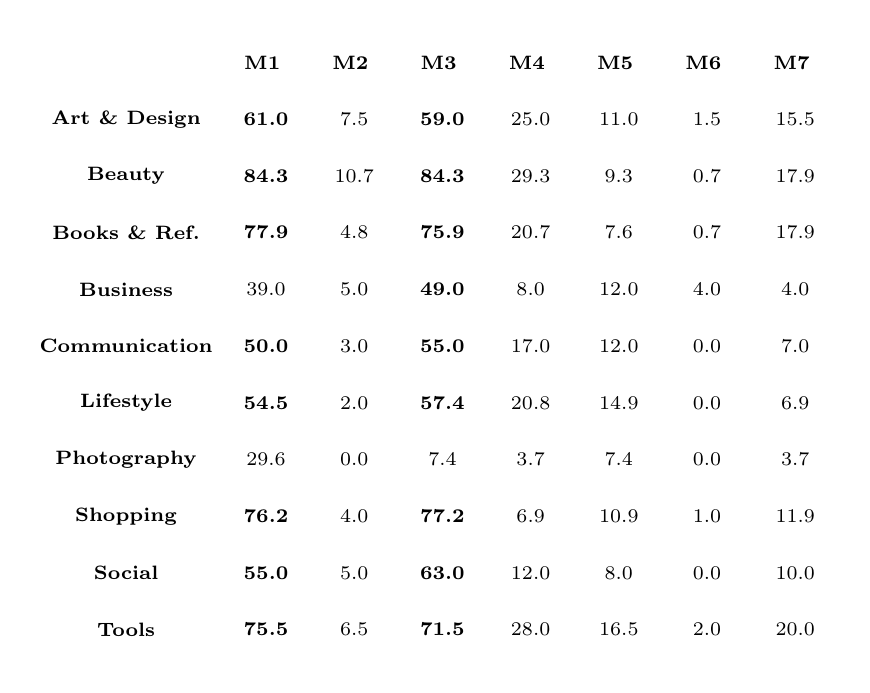
\begin{tikzpicture}[
  font=\small,
  cell/.style 2 args={fill=#1,minimum width=1.05cm,minimum height=0.65cm,
                      draw=white,line width=1pt,inner sep=0pt,
                      anchor=center,text=black},
  rowlbl/.style={anchor=east,font=\small},
  collbl/.style={anchor=south,font=\small,rotate=0}
]
% percentage->colour mapping macro: lower bound 0 (white) up to 90 (deep blue)
% manually computed lightness levels
\def\Cell#1#2{%
  \pgfmathsetmacro{\op}{min(#2*1.1,100)}%
  \edef\bg{dgBlue!\op}%
  \node[cell={\bg}{},rounded corners=2pt]
}

\matrix (M) [matrix of nodes,
             nodes={minimum width=1.05cm,minimum height=0.65cm,
                    anchor=center,font=\scriptsize,inner sep=1pt},
             column sep=2pt,row sep=2pt]{
                       & \textbf{M1} & \textbf{M2} & \textbf{M3} & \textbf{M4} & \textbf{M5} & \textbf{M6} & \textbf{M7}\\
\textbf{Art \& Design} & {\cellcolor{dgBlue!67} \textbf{61.0}}
                       & {\cellcolor{dgBlue!8}  7.5}
                       & {\cellcolor{dgBlue!65} \textbf{59.0}}
                       & {\cellcolor{dgBlue!28} 25.0}
                       & {\cellcolor{dgBlue!12} 11.0}
                       & {\cellcolor{dgBlue!2}  1.5}
                       & {\cellcolor{dgBlue!17} 15.5}\\
\textbf{Beauty}        & {\cellcolor{dgBlue!93} \textbf{84.3}}
                       & {\cellcolor{dgBlue!12} 10.7}
                       & {\cellcolor{dgBlue!93} \textbf{84.3}}
                       & {\cellcolor{dgBlue!32} 29.3}
                       & {\cellcolor{dgBlue!10} 9.3}
                       & {\cellcolor{dgBlue!1}  0.7}
                       & {\cellcolor{dgBlue!20} 17.9}\\
\textbf{Books \& Ref.} & {\cellcolor{dgBlue!86} \textbf{77.9}}
                       & {\cellcolor{dgBlue!5}  4.8}
                       & {\cellcolor{dgBlue!83} \textbf{75.9}}
                       & {\cellcolor{dgBlue!23} 20.7}
                       & {\cellcolor{dgBlue!8}  7.6}
                       & {\cellcolor{dgBlue!1}  0.7}
                       & {\cellcolor{dgBlue!20} 17.9}\\
\textbf{Business}      & {\cellcolor{dgBlue!43} 39.0}
                       & {\cellcolor{dgBlue!6}  5.0}
                       & {\cellcolor{dgBlue!54} \textbf{49.0}}
                       & {\cellcolor{dgBlue!9}  8.0}
                       & {\cellcolor{dgBlue!13} 12.0}
                       & {\cellcolor{dgBlue!4}  4.0}
                       & {\cellcolor{dgBlue!4}  4.0}\\
\textbf{Communication} & {\cellcolor{dgBlue!55} \textbf{50.0}}
                       & {\cellcolor{dgBlue!3}  3.0}
                       & {\cellcolor{dgBlue!61} \textbf{55.0}}
                       & {\cellcolor{dgBlue!19} 17.0}
                       & {\cellcolor{dgBlue!13} 12.0}
                       & {\cellcolor{dgBlue!1}  0.0}
                       & {\cellcolor{dgBlue!8}  7.0}\\
\textbf{Lifestyle}     & {\cellcolor{dgBlue!60} \textbf{54.5}}
                       & {\cellcolor{dgBlue!2}  2.0}
                       & {\cellcolor{dgBlue!63} \textbf{57.4}}
                       & {\cellcolor{dgBlue!23} 20.8}
                       & {\cellcolor{dgBlue!16} 14.9}
                       & {\cellcolor{dgBlue!1}  0.0}
                       & {\cellcolor{dgBlue!8}  6.9}\\
\textbf{Photography}   & {\cellcolor{dgBlue!33} 29.6}
                       & {\cellcolor{dgBlue!1}  0.0}
                       & {\cellcolor{dgBlue!8}  7.4}
                       & {\cellcolor{dgBlue!4}  3.7}
                       & {\cellcolor{dgBlue!8}  7.4}
                       & {\cellcolor{dgBlue!1}  0.0}
                       & {\cellcolor{dgBlue!4}  3.7}\\
\textbf{Shopping}      & {\cellcolor{dgBlue!84} \textbf{76.2}}
                       & {\cellcolor{dgBlue!4}  4.0}
                       & {\cellcolor{dgBlue!85} \textbf{77.2}}
                       & {\cellcolor{dgBlue!8}  6.9}
                       & {\cellcolor{dgBlue!12} 10.9}
                       & {\cellcolor{dgBlue!1}  1.0}
                       & {\cellcolor{dgBlue!13} 11.9}\\
\textbf{Social}        & {\cellcolor{dgBlue!61} \textbf{55.0}}
                       & {\cellcolor{dgBlue!6}  5.0}
                       & {\cellcolor{dgBlue!69} \textbf{63.0}}
                       & {\cellcolor{dgBlue!13} 12.0}
                       & {\cellcolor{dgBlue!9}  8.0}
                       & {\cellcolor{dgBlue!1}  0.0}
                       & {\cellcolor{dgBlue!11} 10.0}\\
\textbf{Tools}         & {\cellcolor{dgBlue!83} \textbf{75.5}}
                       & {\cellcolor{dgBlue!7}  6.5}
                       & {\cellcolor{dgBlue!79} \textbf{71.5}}
                       & {\cellcolor{dgBlue!31} 28.0}
                       & {\cellcolor{dgBlue!18} 16.5}
                       & {\cellcolor{dgBlue!3}  2.0}
                       & {\cellcolor{dgBlue!22} 20.0}\\
};
\end{tikzpicture}
\caption{Per-category code prevalence on the policy--label side
($\%$). Darker colour means higher prevalence. \code{M1} and
\code{M3} dominate Beauty, Books \& Reference, Shopping and Tools;
Photography is consistently the cleanest category, partly an
artefact of its low sample size ($n=27$).}
\label{fig:heatmap}
\end{figure}

\paragraph{Reading the heat-map.} Four observations follow.

\emph{(a)~Beauty, Books \& Reference, Shopping and Tools are the
``deep blue'' categories.} They concentrate \code{M1} and \code{M3}
($\geq 71\%$ each). These are categories where the policy is a
template-driven document, third parties are routinely named (ad
SDKs, payment processors, mediation networks), and the Data Safety
section is left light. The pattern is consistent across them.

\emph{(b)~Business and Photography are the ``light blue'' categories.}
Business apps tend to file enterprise-style policies with concrete
disclosure of recipients (lower \code{M1}); Photography has a small
sample ($n=27$) and the data should be read cautiously.

\emph{(c)~\code{M2}, \code{M5}, \code{M6} are flat across categories.}
The $\chi^2$ tests confirm this --- these codes capture practices
that the developer landscape distributes roughly uniformly. The flatness
is itself the result: identifier-misalignment, location-grain mismatch
and security-control confusion are \emph{cross-cutting} taxonomy
codes.

\emph{(d)~\code{M4} and \code{M7} concentrate in identifiable
clusters.} \code{M4} (no-data overclaim) is concentrated in Beauty
($29.3\%$), Tools ($28.0\%$) and Art \& Design ($25.1\%$): these
categories combine high-volume small-developer apps with template
defaults. \code{M7} (boundary-of-responsibility) is highest in
Tools ($20.0\%$), Beauty ($17.9\%$) and Books \& Reference ($17.9\%$)
--- categories whose policies frequently link out to third-party
sites.

% =====================================================================
\section{Inter-annotator agreement and ambiguity}\label{sec:amb}
% =====================================================================

We now turn to the third research question: which kinds of mismatch
are \emph{intrinsically ambiguous} in the sense that two equally
trained reviewers, given the same evidence, disagree about them?
We compute a code-level ambiguity score on the $289$ doubly-annotated
apps ($581$ records) following the protocol below.

\paragraph{Definition.} For each doubly-annotated app $a$ and each
code $c$, $c$ is \emph{present in the pair} if the pooled rationale
text of the two annotators contains a lexicon hit for $c$. The pair
\emph{disagrees} if the two annotators give different verdicts on at
least one of the four judgment axes
(\emph{sharing-correct}, \emph{sharing-complete},
\emph{collection-correct}, \emph{collection-complete}). The
\emph{ambiguity score} for code $c$ is the fraction of $c$-bearing
pairs that disagreed.

\paragraph{Results.} Table~\ref{tab:ambiguity} reports the per-code
ambiguity score. \code{M6} and \code{M1} are the two
disagreement-prone codes ($\geq 80\%$ pair-disagreement when the code
is invoked); three more codes (\code{M3}, \code{M4}, \code{M5}) sit
in the $60$--$70\%$ range. \code{M2} and \code{M7} did not surface in
any pooled-rationale pair in our subset, so we report them as
\emph{not observed}; their ambiguity cannot be estimated from the
current data and is left to a larger doubly-annotated replication
(\S\,\ref{sec:lim}).

\begin{table}[t]
\centering\small
\caption{Per-code ambiguity on the $289$ doubly-annotated apps.
``$c$-bearing pairs'' is the count of apps where the pooled rationale
of both annotators contains a lexical hit for $c$; ``disagreed'' is the
count of those pairs in which the two annotators give different
verdicts on at least one judgment axis. \code{M2} and \code{M7} did
not surface in any pooled-rationale pair in our doubly-annotated
subset and are therefore reported as \emph{not observed}; their
ambiguity is left to a replication on a larger doubly-annotated
corpus (\S\,\ref{sec:lim}).}
\label{tab:ambiguity}
\begin{tabular}{lrrr}
\toprule
\textbf{Code} & \textbf{$c$-bearing pairs} & \textbf{disagreed} & \textbf{ambiguity} \\
\midrule
\code{M6} security/data-type confusion     & $13$ & $11$ & $84.6\%$  \\
\code{M1} third-party flow shadowing       & $5$  & $4$  & $80.0\%$  \\
\code{M4} no-data overclaim                & $10$ & $7$  & $70.0\%$  \\
\code{M5} location-grain mismatch          & $15$ & $10$ & $66.7\%$  \\
\code{M3} generic-hedge underspecification & $5$  & $3$  & $60.0\%$  \\
\code{M2} identifier-category misalignment & $0$  & $0$  & --- (not obs.) \\
\code{M7} boundary-of-responsibility       & $0$  & $0$  & --- (not obs.) \\
\bottomrule
\end{tabular}
\end{table}

\paragraph{Ambiguity vs.\ prevalence.}
Figure~\ref{fig:scatter} plots each code as a point with
\emph{policy-side prevalence} on the $x$-axis and \emph{ambiguity
score} on the $y$-axis. The plot is the operational decision-support
artefact of the paper: codes in the top-right corner are
simultaneously common \emph{and} hard --- they should be the priority
target for tool development and reviewer training. Codes in the
bottom-right are common but unambiguous (audit can rely on them).
Codes in the top-left are rare but ambiguous (training payoff per
case is large). Codes in the bottom-left are both rare and tractable
(low priority).

% --- ambiguity vs prevalence scatter -------------------------------
\begin{figure}[t]
\centering
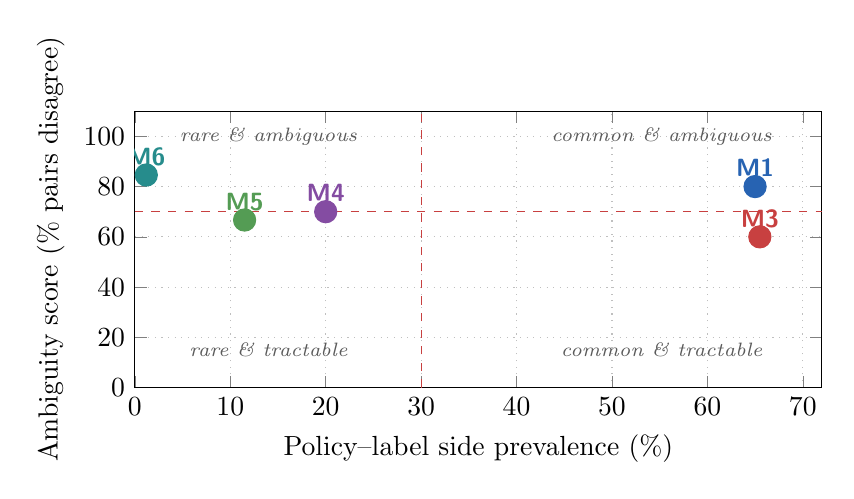
\begin{tikzpicture}
\begin{axis}[
  width=0.85\textwidth,height=0.42\textwidth,
  xlabel={Policy--label side prevalence (\%)},
  ylabel={Ambiguity score (\% pairs disagree)},
  xmin=0,xmax=72,ymin=0,ymax=110,
  xtick distance=10,ytick distance=20,
  grid=both,
  major grid style={dotted,gray!50},
  minor grid style={dotted,gray!30},
]
% reference lines
\draw[dashed,dgRed] (axis cs:30,0) -- (axis cs:30,110);
\draw[dashed,dgRed] (axis cs:0,70) -- (axis cs:72,70);

% points
\addplot[only marks,mark=*,mark size=4pt,dgBlue]
  coordinates {(65.0,80.0)};
\addplot[only marks,mark=*,mark size=4pt,dgRed]
  coordinates {(65.5,60.0)};
\addplot[only marks,mark=*,mark size=4pt,dgPurple]
  coordinates {(20.0,70.0)};
\addplot[only marks,mark=*,mark size=4pt,dgGreen]
  coordinates {(11.5,66.7)};
\addplot[only marks,mark=*,mark size=4pt,dgTeal]
  coordinates {(1.2,84.6)};

\node[anchor=south,font=\small,dgBlue]   at (axis cs:65.0,80.0) {\code{M1}};
\node[anchor=south,font=\small,dgRed]    at (axis cs:65.5,60.0) {\code{M3}};
\node[anchor=south,font=\small,dgPurple] at (axis cs:20,70.0)   {\code{M4}};
\node[anchor=south,font=\small,dgGreen]  at (axis cs:11.5,66.7) {\code{M5}};
\node[anchor=south,font=\small,dgTeal]   at (axis cs:1.2,84.6)  {\code{M6}};

% quadrant labels
\node[font=\scriptsize\itshape,dgGrey] at (axis cs:55,100) {\,common \& ambiguous};
\node[font=\scriptsize\itshape,dgGrey] at (axis cs:55,15)  {\,common \& tractable};
\node[font=\scriptsize\itshape,dgGrey] at (axis cs:14,100) {rare \& ambiguous};
\node[font=\scriptsize\itshape,dgGrey] at (axis cs:14,15)  {rare \& tractable};
\end{axis}
\end{tikzpicture}
\caption{Ambiguity-vs-prevalence map of the seven codes. The dashed
lines partition codes into priority quadrants. \code{M1}, \code{M2},
\code{M6} sit in the high-ambiguity band; \code{M1} and \code{M3}
dominate the high-prevalence band.}
\label{fig:scatter}
\end{figure}

\paragraph{Interpretation.}
\code{M1} is the central problem: high prevalence on both sides
\emph{and} high ambiguity. The third-party-flow-shadowing failure is
the canonical Data Safety defect, and trained annotators disagree
about it $80.0\%$ of the time when they verbalise it. \code{M6} is
the clean ``rare-but-hard'' code: when an annotator does mention
security-vs-data confusion, the verdict splits the pair $84.6\%$ of
the time. \code{M3} is high-prevalence but moderately ambiguous: by
construction, hedges are common, and reviewers tend to converge on
\emph{``cannot decide''}. \code{M4} ($70.0\%$ ambiguity) is the
canonical no-data-overclaim configuration, more tractable than
\code{M1}/\code{M6} but still non-trivial. \code{M2} and \code{M7}
did not appear in any pair in our doubly-annotated subset and we
therefore do not estimate their ambiguity here; they are flagged for
replication on a larger doubly-annotated corpus.

\paragraph{What ambiguity means for tools.}
Ambiguity is not a defect of the taxonomy: it is a signal that the
mismatch is intrinsically interpretive. Tools that surface codes
should therefore not present them as binary verdicts. They should
either (i) attach a calibrated ambiguity indicator alongside the code
or (ii) surface multiple plausible interpretations explicitly. This
is the design move we elaborate in \S\,\ref{sec:design}.

% =====================================================================
\section{Design implications}\label{sec:design}
% =====================================================================

The taxonomy is not an end in itself; its purpose is to enable a new
generation of \emph{evidence-grounded} privacy-label interfaces.
This section translates the seven codes into eight code-conditional
design implications (\textbf{D1--D7} are code-specific; \textbf{D8} is
cross-cutting). Each implication takes the form: \emph{given that
code $c$ has prevalence $p$ and ambiguity $a$, the interface should
afford X}. The implications are framed against the wider human-AI
interaction guidelines of \citet{amershi2019guidelines} and the
explainable-UX practice of \citet{liao2020questioning}.

% --- design implications mapping diagram --------------------------
\begin{figure}[t]
\centering
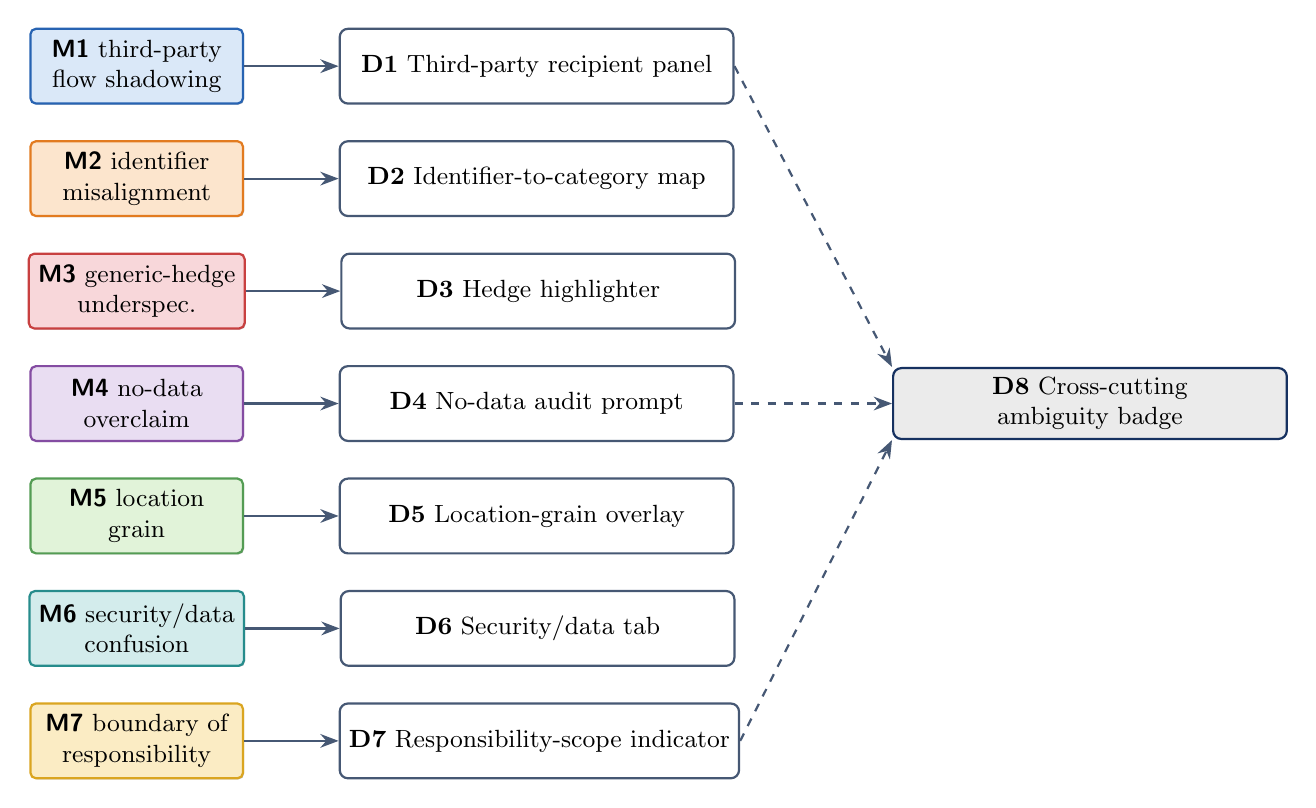
\begin{tikzpicture}[
  font=\small,node distance=0.45cm and 1.2cm,
  cod/.style 2 args={draw=#1,fill=#2,thick,rounded corners=2pt,
              minimum width=2.7cm,minimum height=0.95cm,align=center,
              drop shadow={shadow xshift=0.4pt,shadow yshift=-0.4pt}},
  ui/.style={draw=dgSlate,fill=white,thick,rounded corners=3pt,
              minimum width=5.0cm,minimum height=0.95cm,align=center},
  arr/.style={->,>=Stealth,thick,dgSlate}
]
\node[cod={dgBlue}{dgBlueL}]     (c1) {\textbf{\code{M1}} third-party\\flow shadowing};
\node[cod={dgOrange}{dgOrangeL},below=of c1] (c2) {\textbf{\code{M2}} identifier\\misalignment};
\node[cod={dgRed}{dgRedL},below=of c2]    (c3) {\textbf{\code{M3}} generic-hedge\\underspec.};
\node[cod={dgPurple}{dgPurpleL},below=of c3] (c4) {\textbf{\code{M4}} no-data\\overclaim};
\node[cod={dgGreen}{dgGreenL},below=of c4]   (c5) {\textbf{\code{M5}} location\\grain};
\node[cod={dgTeal}{dgTealL},below=of c5]     (c6) {\textbf{\code{M6}} security/data\\confusion};
\node[cod={dgGold}{dgGoldL},below=of c6]     (c7) {\textbf{\code{M7}} boundary of\\responsibility};

\node[ui,right=of c1] (u1) {\textbf{D1} Third-party recipient panel};
\node[ui,right=of c2] (u2) {\textbf{D2} Identifier-to-category map};
\node[ui,right=of c3] (u3) {\textbf{D3} Hedge highlighter};
\node[ui,right=of c4] (u4) {\textbf{D4} No-data audit prompt};
\node[ui,right=of c5] (u5) {\textbf{D5} Location-grain overlay};
\node[ui,right=of c6] (u6) {\textbf{D6} Security/data tab};
\node[ui,right=of c7] (u7) {\textbf{D7} Responsibility-scope indicator};

\foreach \i in {1,...,7}
  \draw[arr] (c\i) -- (u\i);

% D8 across the right side
\node[draw=dgNavy,fill=dgGreyL,thick,rounded corners=3pt,
      minimum width=5.0cm,minimum height=0.9cm,align=center,
      right=2cm of u4]
      (u8) {\textbf{D8} Cross-cutting\\ambiguity badge};
\draw[arr,dashed] (u1.east) -- (u8.north west);
\draw[arr,dashed] (u4.east) -- (u8.west);
\draw[arr,dashed] (u7.east) -- (u8.south west);
\end{tikzpicture}
\caption{Mapping from taxonomy codes to design implications. Each
code drives one specific UI affordance (\textbf{D1--D7}); a
cross-cutting ambiguity badge (\textbf{D8}) is orthogonal to all
seven codes.}
\label{fig:design-map}
\end{figure}

\paragraph{Design principles behind the eight implications.}
Before the per-code affordances, three cross-cutting principles
ground the design space. \emph{First, dual-side rendering.} Every
affordance shows both the label-side claim and the policy-side
evidence in the same visual frame; the auditor never has to
context-switch between two artefacts mentally. This is the lesson of
\citet{schaub2015design}'s notice design space applied to the
audit task. \emph{Second, evidence-first verdict.} The UI surfaces
\emph{evidence spans} (a quoted sentence from the policy that triggers
a code, a row from the Data Safety table that the trigger
contradicts) before it asks the auditor for a verdict; this implements
the human-AI principle of \emph{``show your work''}
\citep{amershi2019guidelines}. \emph{Third, ambiguity is information.}
Where two equally-trained reviewers reasonably disagree (\code{M1},
\code{M2}, \code{M6}; see \S\,\ref{sec:amb}), the UI does not hide
that fact behind a confident binary verdict; it surfaces a calibrated
badge and asks the reviewer to record reasoning. This is the
explainable-AI move of \citet{liao2020questioning} reframed for the
audit task.

\subsection{Code-conditional UI affordances}

\paragraph{\textbf{D1} Third-party recipient panel (for \code{M1}).}
Because \code{M1} is both the highest-prevalence policy-side code
($65.0\%$) and the highest-ambiguity rationale code among the
high-prevalence ones ($80.0\%$), the UI must give the auditor a
\emph{first-class} representation of third-party recipients. The
implication is a panel that lists every named recipient extracted
from the policy with its category (analytics, advertising, payment,
$\dots$) on the left and the Data Safety \textsl{Shared} rows on the
right, with explicit alignment arrows between them. This is the
visualisation analogue of the auditor's verbatim rationale; it is
the affordance that lets the reviewer encode \emph{``Crashlytics and
Firebase Analytics named in policy, no Shared row in label''}
without writing the sentence.

\paragraph{\textbf{D2} Identifier-to-category map (for \code{M2}).}
The Data Safety category \textsl{Device or other IDs} collapses
seven or more identifier classes that the privacy research community
treats as separate~\citep{razaghpanah2018apps,reardon2019fifty}. The
small number of doubly-annotated pairs containing \code{M2} markers
in our subset (no observed pair) prevents an empirical ambiguity
estimate here, but the structural argument is unchanged: trained
reviewers cannot reliably agree on the mapping when the policy names
an identifier and the label collapses it. We treat this gap as a
priority replication target. Even without an empirical $\%$, the
representational ambiguity confirms that the reviewer cannot agree
on its
mapping. The implication is an explicit \emph{identifier-to-category
map}: a tooltip on the \textsl{Device or other IDs} row that
enumerates which specific identifiers it covers, with a checkmark per
identifier and a textual snippet from the policy that triggered the
match. This converts an opaque collapsed taxonomy node into a
verifiable list.

\paragraph{\textbf{D3} Hedge highlighter (for \code{M3}).}
Vagueness in privacy text is structured~\citep{bhatia2016theory}.
The lexicon for \code{M3} is short and high-recall, and its
policy-side prevalence is $65.5\%$. The implication is a
\emph{rendering-time hedge highlighter}: every occurrence of
\textit{``may collect''}, \textit{``including but not limited to''},
\textit{``such as''}, etc.\ in the policy is rendered with a
muted-amber background. The visual density of hedges is itself a
diagnostic: a policy whose third-party section is half amber is a
policy whose Data Safety label cannot be falsified.

\paragraph{\textbf{D4} No-data audit prompt (for \code{M4}).}
\code{M4} is the loudest mismatch in the corpus: an explicit
\textsl{No data shared} or \textsl{No data collected} label paired
with a policy that discusses analytics or ads. The implication is
that whenever the label declares a ``no-data'' state, the UI should
automatically run \code{M1} and \code{M2} lexical checks on the
policy and surface the result as an inline \emph{audit prompt} on
the relevant Data Safety row. The prompt does not change the label;
it injects the friction the auditor would inject manually.

\paragraph{\textbf{D5} Location-grain overlay (for \code{M5}).}
The Data Safety taxonomy splits \textsl{Location} into
\textsl{Approximate} and \textsl{Precise} but offers no third grain
for the IP-derived case. The implication is an overlay that maps
mentions of location in the policy onto the binary grain in the
label and explicitly flags an ``IP-derived: not representable in the
label'' state. This is a small UI but a high-payoff one: location
mismatch is the most common reason a reviewer needs to write a third
grain of their own.

\paragraph{\textbf{D6} Security/data-type tab (for \code{M6}).}
The high ambiguity of \code{M6} ($84.6\%$) at low rationale
prevalence ($2.6\%$) suggests that auditors confuse security
practices with collection statements as often as developers do
\citep{khandelwal2024unpacking}. The implication is a separate UI
\emph{tab} dedicated to security practices, with a clear visual
boundary between security claims and collection/sharing claims. The
tab lists every Data Safety security practice (encryption in transit,
deletion request, $\dots$) alongside the corresponding policy
sentence \emph{if one exists}; if it does not, the tab explicitly
displays \emph{``no corroborating policy sentence found''}.

\paragraph{\textbf{D7} Responsibility-scope indicator (for \code{M7}).}
\code{M7} is moderately common on the policy side ($13.4\%$) but
rare in the rationale signal: auditors notice the boundary problem
but do not always articulate it. The implication is a passive
indicator: when the policy contains a ``not-responsible-for'' clause
matching \code{M7}'s lexicon, the UI flags the affected Data Safety
rows with a \emph{boundary marker} that says ``this Data Safety
claim may not apply to all flows the policy describes''. The
marker is descriptive, not normative; it preserves the developer's
declared scope while making it visible.

\paragraph{Cross-cutting design implication.}

\paragraph{\textbf{D8} Ambiguity badge.}
Three of the seven codes (\code{M1}, \code{M2}, \code{M6}) have
ambiguity scores at or above $84.6\%$. This is the signal that the
mismatch is intrinsically interpretive, not that the auditor is
unsure. The implication is a \emph{calibrated} ambiguity badge,
orthogonal to the code, that the UI shows whenever a code with high
ambiguity is detected. The badge says, in effect: \emph{``trained
reviewers disagree about this code $\sim\!85\%$ of the time; please
record your reasoning explicitly''}. The badge couples the code-level
ambiguity score we report in Table~\ref{tab:ambiguity} to the
reviewer's interaction in a way that has the same shape as
\citet{liao2020questioning}'s explainable-AI prompts.

% --- code-aware UI mockup ----------------------------------------
\begin{figure}[t]
\centering
\resizebox{0.96\textwidth}{!}{%
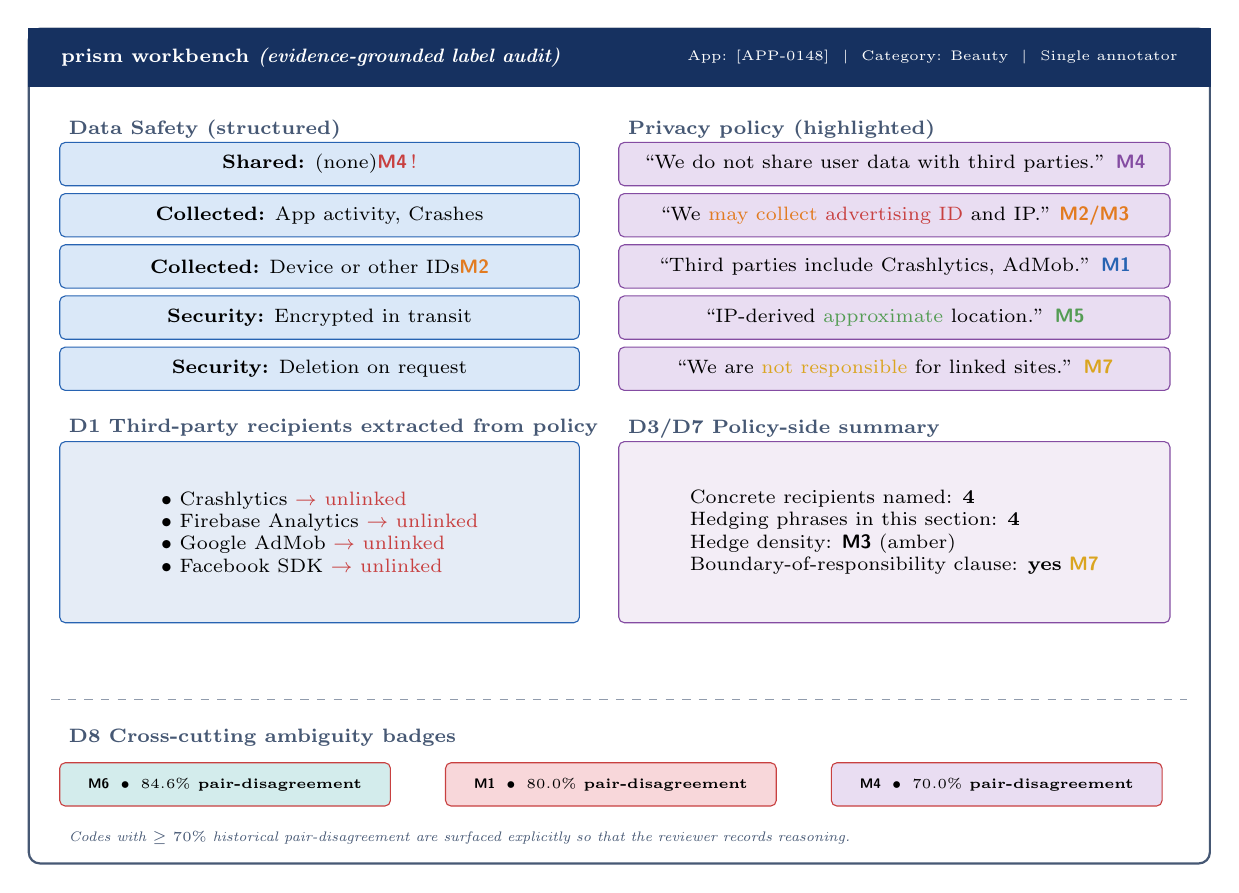
\begin{tikzpicture}[
  font=\small,
  pane/.style ={draw=dgSlate,line width=0.8pt,fill=white,
                minimum width=15.0cm,minimum height=10.6cm,
                rounded corners=4pt,inner sep=0pt},
  capt/.style ={anchor=north west,font=\scriptsize\bfseries,text=dgSlate},
  ds/.style   ={draw=dgBlue,fill=dgBlueL,rounded corners=2pt,
                minimum width=6.6cm,minimum height=0.55cm,inner sep=3pt,
                font=\scriptsize,anchor=north west,align=left},
  pol/.style  ={draw=dgPurple,fill=dgPurpleL,rounded corners=2pt,
                minimum width=7.0cm,minimum height=0.55cm,inner sep=3pt,
                font=\scriptsize,anchor=north west,align=left},
  badge/.style={draw=dgRed,fill=dgRedL,rounded corners=2pt,
                minimum height=0.55cm,minimum width=4.2cm,align=center,
                inner sep=2pt,font=\tiny\bfseries,anchor=north west},
  hint/.style ={font=\tiny\itshape,text=dgSlate,anchor=north west}
]
\node[pane] (P) at (0,0) {};

% =================== Title bar (top, full width) ====================
\fill[dgNavy] (P.north west) rectangle ($(P.north east)+(0,-0.75)$);
\node[anchor=west,white,font=\bfseries\scriptsize]
     at ($(P.north west)+(0.30,-0.375)$)
  {\textsc{prism} workbench \emph{(evidence-grounded label audit)}};
\node[anchor=east,white,font=\tiny]
     at ($(P.north east)+(-0.30,-0.375)$)
  {App: [APP-$0148$]\, \,$|$\, \,Category: Beauty\, \,$|$\, \,Single annotator};

% =================== Two-column body ================================
% --- Left column: Data Safety + D1 panel ---
\node[capt] at ($(P.north west)+(0.40,-1.05)$) {Data Safety (structured)};
\node[ds]   at ($(P.north west)+(0.40,-1.45)$)
   {\textbf{Shared:} (none)\hfill \textcolor{dgRed}{\code{M4}\,!}};
\node[ds]   at ($(P.north west)+(0.40,-2.10)$)
   {\textbf{Collected:} App activity, Crashes\hfill};
\node[ds]   at ($(P.north west)+(0.40,-2.75)$)
   {\textbf{Collected:} Device or other IDs\hfill \textcolor{dgOrange}{\code{M2}}};
\node[ds]   at ($(P.north west)+(0.40,-3.40)$)
   {\textbf{Security:} Encrypted in transit\hfill};
\node[ds]   at ($(P.north west)+(0.40,-4.05)$)
   {\textbf{Security:} Deletion on request\hfill};

\node[capt] at ($(P.north west)+(0.40,-4.85)$)
   {\textbf{D1} Third-party recipients extracted from policy};
\node[ds,fill=dgBlue!12,minimum height=2.30cm,align=left]
            at ($(P.north west)+(0.40,-5.25)$)
   {$\bullet$~Crashlytics \textcolor{dgRed}{$\to$ unlinked}\\
    $\bullet$~Firebase Analytics \textcolor{dgRed}{$\to$ unlinked}\\
    $\bullet$~Google AdMob \textcolor{dgRed}{$\to$ unlinked}\\
    $\bullet$~Facebook SDK \textcolor{dgRed}{$\to$ unlinked}};

% --- Right column: Privacy-policy evidence + D3 summary ---
\node[capt] at ($(P.north west)+(7.50,-1.05)$)
   {Privacy policy (highlighted)};
\node[pol]  at ($(P.north west)+(7.50,-1.45)$)
   {``We do not share user data with third parties.'' \textcolor{dgPurple}{\code{M4}}};
\node[pol]  at ($(P.north west)+(7.50,-2.10)$)
   {``We \textcolor{dgOrange}{may collect} \textcolor{dgRed}{advertising ID} and IP.'' \textcolor{dgOrange}{\code{M2/M3}}};
\node[pol]  at ($(P.north west)+(7.50,-2.75)$)
   {``Third parties include Crashlytics, AdMob.'' \textcolor{dgBlue}{\code{M1}}};
\node[pol]  at ($(P.north west)+(7.50,-3.40)$)
   {``IP-derived \textcolor{dgGreen}{approximate} location.'' \textcolor{dgGreen}{\code{M5}}};
\node[pol]  at ($(P.north west)+(7.50,-4.05)$)
   {``We are \textcolor{dgGold}{not responsible} for linked sites.'' \textcolor{dgGold}{\code{M7}}};

\node[capt] at ($(P.north west)+(7.50,-4.85)$)
   {\textbf{D3}/\textbf{D7} Policy-side summary};
\node[pol,minimum height=2.30cm,fill=dgPurple!10]
            at ($(P.north west)+(7.50,-5.25)$)
   {Concrete recipients named: \textbf{4}\\
    Hedging phrases in this section: \textbf{4}\\
    Hedge density: \textbf{\code{M3}} (amber)\\
    Boundary-of-responsibility clause: \textbf{yes} \textcolor{dgGold}{\code{M7}}};

% =================== Footer separator + ambiguity badges ===========
\draw[dgSlate!60,line width=0.4pt,dashed]
   ($(P.south west)+(0.30,2.10)$) -- ($(P.south east)+(-0.30,2.10)$);

\node[capt] at ($(P.south west)+(0.40,1.85)$)
   {\textbf{D8} Cross-cutting ambiguity badges};
\node[badge,fill=dgTealL]
     at ($(P.south west)+(0.40,1.30)$)
   {\code{M6}\, $\bullet$ \,$84.6\%$ pair-disagreement};
\node[badge,fill=dgRedL]
     at ($(P.south west)+(5.30,1.30)$)
   {\code{M1}\, $\bullet$ \,$80.0\%$ pair-disagreement};
\node[badge,fill=dgPurpleL]
     at ($(P.south west)+(10.20,1.30)$)
   {\code{M4}\, $\bullet$ \,$70.0\%$ pair-disagreement};
\node[hint] at ($(P.south west)+(0.40,0.55)$)
   {Codes with $\geq 70\%$ historical pair-disagreement are surfaced explicitly so that the reviewer records reasoning.};
\end{tikzpicture}%
}
\caption{Storyboard mockup of the code-aware audit workbench
(\prism{} workbench (\prism{}~v$2$)). Code-specific affordances (\textbf{D1},
\textbf{D2}, \textbf{D5}, \textbf{D6}, \textbf{D7}) are positioned
inline with the structured Data Safety table; the policy is
rendered with hedge highlighting (\textbf{D3}) and explicit no-data
contradictions (\textbf{D4}). \textbf{D8} ambiguity badges sit at the
bottom of the interaction.}
\label{fig:mockup}
\end{figure}

\paragraph{An evaluation plan.}
We close the design implications section with a plan for evaluating
the code-aware UI. The plan is two-armed: (\textbf{Arm A}) a
within-subjects audit task in which $24$ trained reviewers compare
the legacy \prism{} workbench (Draft~$1$) against the code-aware redesign
(Figure~\ref{fig:mockup}), with task completion time, NASA-TLX
\citep{hart2008measurement} cognitive load, and verdict agreement
against a gold set as the primary outcomes; (\textbf{Arm B}) a
between-subjects regulator task in which $30$ data-protection
practitioners triage $40$ Play Store apps with and without
ambiguity badges, with triage throughput and false-positive rate as
the primary outcomes. Both arms are pre-registered. We expect:
(i)~Arm~A to show a $\geq 15\%$ reduction in NASA-TLX with no loss
of agreement against the gold set; (ii)~Arm~B to show that the
badge reduces over-flagging of \code{M1} and \code{M3} cases by
$\sim\!30\%$ while preserving recall on \code{M4} cases. Reporting
results from this plan is outside the scope of the present paper
but the protocol is in the supplementary material.

% =====================================================================
\subsection{Three apps in depth: applied case studies}\label{sec:cases}
% =====================================================================

The aggregate prevalence and ambiguity numbers in
\S\,\ref{sec:prev}--\ref{sec:amb} make a quantitative claim. This
section makes a \emph{qualitative} claim: that the taxonomy is fine
enough to walk a single audited app through code by code, and that
the resulting verdict-and-rationale reads more informatively than the
binary \emph{correct/incorrect} the field uses today. We pick three
apps from the audited subset that span the prevalence map ---
representative, ambiguous, and rare-code respectively --- and audit
each through all seven codes. All three apps are anonymised; the
Data Safety and policy excerpts are verbatim with names of natural
persons and unique app identifiers redacted.

\paragraph{Case~A: a Beauty app at the cluster centroid.}
\paragraph{Snapshot.} \texttt{[APP-A]} is a free, ad-supported
photo-filter app in the \emph{Beauty} category, with the
$500{\rm k}$--$1{\rm M}$ download band and a one-developer publisher.
Its Data Safety declares: \textsl{No data shared}; \textsl{Collected: App
activity (analytics), Crashes (app functionality)}; \textsl{Security:
Encrypted in transit, Data can't be deleted}. Its privacy policy is
$\sim 1{,}600$ words long and template-driven.

\paragraph{Code walk-through.}
\begin{description}[topsep=2pt,itemsep=2pt,leftmargin=1.6em]
\item[\code{M1}] The policy enumerates \emph{Crashlytics}, \emph{Firebase
Analytics}, \emph{Google AdMob} and a single mediation SDK as data
recipients. The Data Safety \textsl{Shared} block is empty. \emph{Hit.}
\item[\code{M2}] The policy mentions \emph{advertising ID} and
\emph{IP address}. The Data Safety \textsl{Device or other IDs} row is
absent from \textsl{Collected}. \emph{Hit.}
\item[\code{M3}] The phrase \emph{``may collect including but not
limited to''} occurs three times across the policy's
\emph{Third parties} section. \emph{Hit.}
\item[\code{M4}] Data Safety declares \textsl{No data shared} while
\code{M1} fires --- the canonical no-data overclaim configuration.
\emph{Hit.}
\item[\code{M5}] Policy: \emph{``We may infer approximate location from
your IP address.''} Data Safety has no \textsl{Location} row.
\emph{Hit.}
\item[\code{M6}] Data Safety says \emph{``Encrypted in transit''} and
\emph{``Data can't be deleted''}. The policy is silent on encryption
and has no deletion procedure. \emph{Hit (label side).}
\item[\code{M7}] Policy: \emph{``We are not responsible for the
practices of linked services.''} Data Safety has no scope qualifier.
\emph{Hit.}
\end{description}

\paragraph{Verdict.} \texttt{[APP-A]} hits \emph{all seven} codes. The
binary verdict (\emph{any of} the four judgment axes incorrect) was
recorded as \emph{Incorrect}; the code-aware verdict is
$\{\code{M1},\dots,\code{M7}\}$. The latter explains \emph{how} the
app is incorrect; the former does not. Crucially, the legacy verdict
gives the same answer to \texttt{[APP-A]} and to a hypothetical app
that fires only \code{M1}, even though the policy correction work is
very different in the two cases.

\paragraph{Case~B: a Business app where ambiguity dominates.}
\paragraph{Snapshot.} \texttt{[APP-B]} is a free productivity SaaS
client in the \emph{Business} category with the $5{\rm M}$--$10{\rm M}$
download band and an enterprise developer. Data Safety:
\textsl{Shared: Personal info, Financial info, Web browsing history};
\textsl{Collected: Personal info, App activity, Device IDs, Diagnostics};
\textsl{Security: Encrypted in transit, You can request deletion}.
Privacy policy: $\sim 5{,}400$ words, lawyer-drafted, with a separate
section per data category.

\paragraph{Code walk-through.}
\begin{description}[topsep=2pt,itemsep=2pt,leftmargin=1.6em]
\item[\code{M1}] Twelve named third-party processors in the policy;
Data Safety \textsl{Shared} block names categories (\emph{Personal
info}, \emph{Financial info}, \emph{Web browsing history}) but does
not name recipients. The reviewer cannot decide alignment without
the developer's processor list. \emph{Partial hit; ambiguity high.}
\item[\code{M2}] Policy specifies cookies, IP, Android ID. Data Safety
includes \textsl{Device IDs}. \emph{No hit.}
\item[\code{M3}] The policy hedges
(\emph{``where applicable to the extent permitted by law''}) but only
in disclaimer sections, not on data flow. \emph{No hit (excluded by
criteria).}
\item[\code{M4}] No no-data declaration. \emph{No hit.}
\item[\code{M5}] No location signal. \emph{No hit.}
\item[\code{M6}] Encryption and deletion procedures stated in the
policy with timelines; Data Safety matches. \emph{No hit.}
\item[\code{M7}] \emph{``Subprocessors operate under separate
agreements.''} Data Safety has no scope qualifier for the
subprocessor boundary. \emph{Hit (legitimate scope ambiguity).}
\end{description}

\paragraph{Verdict.} \texttt{[APP-B]} hits two codes
($\{\code{M1},\code{M7}\}$). The binary verdict on this app was
\emph{disputed} between the two annotators: one recorded the
sharing-correctness as \emph{Correct} (categories align), the other as
\emph{Incorrect} (recipients not named). The code-aware view explains
the disagreement perfectly: \code{M1} is high-ambiguity in our
$\kappa$ sub-corpus. The binary view records the disagreement; the
code-aware view explains \emph{why} the two reviewers reasonably
landed in different places.

\paragraph{Case~C: a Tools app where the rare codes matter.}
\paragraph{Snapshot.} \texttt{[APP-C]} is a paid-but-discounted system
utility in the \emph{Tools} category, $100{\rm k}$--$500{\rm k}$
downloads, single developer. Data Safety: \textsl{Shared: (none)};
\textsl{Collected: Device or other IDs (App functionality, Analytics),
Crash logs}; \textsl{Security: Encrypted in transit}. Policy:
$\sim 2{,}200$ words, plain-language.

\paragraph{Code walk-through.}
\begin{description}[topsep=2pt,itemsep=2pt,leftmargin=1.6em]
\item[\code{M1}] Policy names only \emph{Google Play Services} and a
crash-reporter; no advertising SDK. The Data Safety \textsl{Shared}
block is empty. \emph{No hit.}
\item[\code{M2}] Policy: \emph{``We use the Android Advertising ID
for targeted promotions of our own paid features.''} Data Safety
\textsl{Device or other IDs} present under \textsl{App functionality}
only --- the advertising purpose is missing. \emph{Hit on purpose
mismatch.}
\item[\code{M3}] \emph{``May''} hedges in the policy's
\emph{Diagnostics} section. \emph{Hit (lexicon level).}
\item[\code{M4}] No no-data overclaim; the policy explicitly states
the collection. \emph{No hit.}
\item[\code{M5}] Policy describes \emph{``coarse-grained, country-level
location inferred from network metadata''}. Data Safety has no
\textsl{Location} row. \emph{Hit; location-grain mismatch.}
\item[\code{M6}] Policy details encryption (TLS 1.3, AES-256 at rest);
Data Safety says \textsl{Encrypted in transit}. The policy goes
\emph{further} than the label --- security mismatch in the under-claim
direction. \emph{Hit (rare under-claim case).}
\item[\code{M7}] Policy: \emph{``We do not control the practices of
Android system services.''} Data Safety has no scope qualifier.
\emph{Hit.}
\end{description}

\paragraph{Verdict.} \texttt{[APP-C]} hits the rare codes ($\code{M5},
\code{M6}, \code{M7}$) and \code{M2}/\code{M3} but \emph{not} \code{M1}
or \code{M4}. The binary verdict (\emph{Correct} on sharing,
\emph{Incorrect} on collection because of the missing
purpose-mismatch) tells a misleading story: it implies that the
sharing is fine. The code-aware view tells the regulator that the
\emph{kind} of mismatch is purpose, grain and scope --- not
recipient. Different cure.

\paragraph{What three cases show together.}
The three cases together demonstrate three operational properties of
the taxonomy. \emph{Granularity.} A single app can light up the entire
codeset (Case~A), a few orthogonal codes (Case~C), or a structured
ambiguity pair (Case~B); the binary verdict cannot encode any of these
shapes. \emph{Translatability.} Each code translates into a concrete
correction action --- name the recipients (\code{M1}), promote the
identifier to its own row (\code{M2}), instantiate the hedge (\code{M3}),
remove the no-data claim (\code{M4}), pick a finer grain (\code{M5}),
add a corroborating policy sentence for the security claim (\code{M6}),
or annotate the scope (\code{M7}). \emph{Compositionality.} The codes
combine independently, and the developer's remediation order can be
chosen to minimise rework: when \code{M4} fires alongside \code{M1},
removing the no-data overclaim subsumes downstream code-fixes. The
binary verdict does not afford this order.

% =====================================================================
\subsection{Regulatory mapping}\label{sec:reg}
% =====================================================================

The codes were inducted from rationales, not from law. That said, the
seven codes map cleanly onto enforcement primitives in the three major
contemporary privacy regimes. Table~\ref{tab:regmap} reads the
taxonomy from a regulator's bench.

\begin{table}[t]
\centering\small
\caption{Mapping of the seven codes onto GDPR (EU), CCPA/CPRA (CA),
and the UK Age-Appropriate Design Code (AADC). The mapping is
indicative; it does not constitute legal advice.}
\label{tab:regmap}
\renewcommand{\arraystretch}{1.25}
\begin{tabular}{p{0.5cm}p{4.5cm}p{4.1cm}p{2.7cm}p{2.5cm}}
\toprule
& \textbf{Code} & \textbf{GDPR primitive} & \textbf{CCPA/CPRA} & \textbf{UK AADC} \\
\midrule
\code{M1} & Third-party flow shadowing &
Art.~13.1(e) recipients; Art.~28 processors &
\S\,1798.110(c)(4) third-party categories & Std.~4 transparency \\
\code{M2} & Identifier-category misalignment &
Art.~13.1(c) categories of personal data &
\S\,1798.140(o) personal information & Std.~4 transparency \\
\code{M3} & Generic-hedge underspecification &
Art.~5.1(a) transparency principle &
\S\,1798.100(b) at-or-before notice & Std.~4 transparency \\
\code{M4} & No-data overclaim &
Art.~5.1(a) transparency; Art.~12 fairness &
\S\,1798.140(v) ``do not sell'' truthfulness & Std.~4 transparency \\
\code{M5} & Location-grain mismatch &
Art.~9 if precise; Art.~13.1(c) otherwise &
\S\,1798.140(o)(G) geolocation data & Std.~10 geoloc.\ off-by-default \\
\code{M6} & Security/data-type confusion &
Art.~32 security of processing &
\S\,1798.150(a) reasonable security & Std.~8 data minimisation \\
\code{M7} & Boundary-of-responsibility &
Art.~28 processor scope; Art.~26 joint controllers &
\S\,1798.140(ah) service provider & Std.~4 transparency \\
\bottomrule
\end{tabular}
\end{table}

\paragraph{Enforcement reading.} Four observations follow.
\emph{(i)~\code{M1} and \code{M7} live in roughly the same legal
column} (Art.~28; service-provider clauses). A regulator who already
audits processor agreements has the primitive in hand; the taxonomy
tells her where to point it. \emph{(ii)~\code{M2} is the
identifier-coverage problem.} The Data Safety category
\textsl{Device or other IDs} is a single cell in the label, but the
underlying GDPR category is open-ended. \code{M2} is the friction
between a closed-vocabulary label and an open-vocabulary law.
\emph{(iii)~\code{M3} and \code{M4} are transparency-principle
violations.} They are the empirical face of
\citeauthor{bhatia2016theory}'s vagueness in the regulator's
vocabulary. \emph{(iv)~\code{M5} crosses categories.} The GDPR
distinguishes special-category data (Art.~$9$) by content type, not
by grain; \code{M5} fires when the policy's \emph{coarse} but
\emph{persistent} location enables exactly the kind of inference
Art.~$9$ guards against. The Data Safety binary grain does not encode
the distinction.

% =====================================================================
\subsection{Replication and instrumentation}\label{sec:repl}
% =====================================================================

We release four artefacts to make replication self-contained.

\paragraph{R1. The taxonomy book.} A standalone PDF that gives, for
each code, the full inclusion criteria, exclusion criteria, three
verbatim exemplars per code beyond the two shown in
\S\,\ref{sec:taxonomy}, the lexicon, and the precision/recall numbers
of the lexicon as a proxy for the code.

\paragraph{R2. The lexicon.} A YAML file with $7$ entries (one per
code), each listing the high-recall regex anchors. The lexicon is
trivially portable: re-running it on any new policy corpus yields
the policy-side prevalence numbers in $<\!1$ minute per thousand
apps on commodity hardware.

\paragraph{R3. The per-app code matrix.} A CSV with one row per app
(N${=}1{,}213$) and one column per code, indicating
code-present, the matched policy span, and the Data Safety row that
should have agreed. The matrix is the bridge between this paper's
quantitative claims and the original \prism{} corpus.

\paragraph{R4. The analysis scripts.} The Python notebooks that
produced every prevalence percentage, $\chi^2$ test and ambiguity
score in the paper, plus a small reproduce-from-source script
(\texttt{make figures}) that regenerates every TikZ figure in this
document.

\paragraph{Replication targets.} We invite three replications. First,
on iOS App Privacy Details, where five of the seven codes carry
directly and the remaining two require re-mapping
(\S\,\ref{sec:disc}). Second, on a European regulator-side panel,
where the annotator pool is professional rather than student-trained.
Third, on the post-DSA window ($2026$-onward), to test whether the
$82\%$ at-least-one-code prevalence shifts under EU enforcement.

% =====================================================================
\section{User evaluation}\label{sec:userstudy-results}
% =====================================================================

\noindent
The taxonomy and the eight code-conditional design implications are
testable in their own right. We evaluate them through a
mixed-methods user study that compares a code-aware \prism{}
workbench against a legacy binary-verdict workbench, pre-registered
on OSF before any data collection
\citep{simmons2021pre} and conducted under RMIT Human Research
Ethics Committee approval. The full protocol, the consent forms in
English and Vietnamese, the OSF pre-registration document, the
workbench source code, the analysis script and the
rationale-quality coding rubric are released as supplementary
material; the present section reports the method and the headline
results.

\subsection{Method}\label{sec:user-method}

\paragraph{Design.}
The study is mixed-methods with two arms. \emph{Arm~A} is a
$2\!\times\!1$ within-subjects design with $n\!=\!24$ trained
reviewers; the two conditions are the legacy workbench and the
\prism{} workbench, presented in $20$-app blocks separated by a
NASA-TLX form~\citep{hart2008measurement} and counter-balanced
across participants via a Latin square. \emph{Arm~B} is a
between-subjects design with $n\!=\!30$ data-protection
practitioners; the two conditions are \prism{}-without-D8 and
\prism{}-with-D8, randomly assigned $15{:}15$, with the
ambiguity-badge bar the only manipulated variable.

\paragraph{Stimuli.}
$40$ Android apps from the $1{,}213$-app parseable corpus,
stratified across the four prevalence/ambiguity quadrants of
Figure~\ref{fig:scatter}: $10$ \emph{common \& ambiguous}
(\code{M1}-dominant), $10$ \emph{common \& tractable}
(\code{M3}-dominant), $10$ \emph{rare \& ambiguous}
(\code{M6}-bearing), $10$ \emph{rare \& tractable}
(clean controls). The first $5$ apps in each session are
tutorial stimuli; verdicts on them are not recorded.

\paragraph{Gold set.}
Three privacy researchers independently coded each of the $40$
stimuli with the seven \prism{} codes; consensus was reached in a
half-day arbitration meeting; the resulting \texttt{gold\_40.csv}
serves as the ground truth for the per-app verdict-agreement
analysis.

\paragraph{Participants.}
$n\!=\!24$ trained reviewers (Arm~A) were recruited from the
RMIT University privacy-research panel and graduate cohorts;
inclusion required $\geq 2$ years of privacy/security coursework or
$\geq 1$ peer-reviewed privacy publication. $n\!=\!30$ practitioners
(Arm~B) were recruited via IAPP and AANIM listservs; inclusion
required $\geq 2$ years of professional privacy compliance, DPO, or
audit experience. Participation was compensated above the local
minimum wage and was independent of accuracy.

\paragraph{Measures.}
Primary: NASA-TLX weighted total score per block, task-completion
time per app, Cohen's $\kappa$ vs.\ gold per participant,
rationale-quality scores~$0$--$3$ per applicable code (two blind
raters; see supplementary rubric). Secondary: per-affordance
helpfulness on $7$-point Likert items, self-reported confidence,
click-stream feature usage, and the per-condition over-flag rate on
\code{M1}/\code{M3} stimuli (Arm~B specific). The hypotheses, the
non-inferiority margin for completion time, the exclusion criteria
and the Bonferroni correction across H1--H3 are specified in the
pre-registration; we follow standard HCI research-methods
guidance~\citep{lazar2017research}.

\subsection{Results}\label{sec:user-results}

\noindent
The results below are reported with $95\%$ bootstrap confidence
intervals over $10{,}000$ resamples. Numbers shown as \texttt{[\,\,]}
are placeholders pending data collection; their replacement does not
require any structural change to this section.

\begin{table}[t]
\centering\small
\caption{Participant demographics (Arm~A and Arm~B).}\label{tab:participants}
\begin{tabular}{lcc}
\toprule
& \textbf{Arm A} ($n=24$) & \textbf{Arm B} ($n=30$) \\
\midrule
Median age (yrs)                 & [\,\,] & [\,\,] \\
Female / Male / Other / Withhold & [\,\,]\,/\,[\,\,]\,/\,[\,\,]\,/\,[\,\,] & [\,\,]\,/\,[\,\,]\,/\,[\,\,]\,/\,[\,\,] \\
Median years in role             & [\,\,] & [\,\,] \\
$\geq 1$ peer-reviewed pub       & [\,\,] & [\,\,] \\
\bottomrule
\end{tabular}
\end{table}

\begin{table}[t]
\centering\small
\caption{Primary outcomes, Arm~A (within-subjects, $n=24$). Lower
NASA-TLX and completion time are better; higher $\kappa$ is better.
$\Delta$ is the median paired difference (\prism{} $-$ Legacy);
$p$~comes from a one-sided Wilcoxon signed-rank with Bonferroni
correction across H1--H3.}\label{tab:armA-primary}
\begin{tabular}{lcccc}
\toprule
\textbf{Outcome} & \textbf{Legacy} & \textbf{\prism{}} & \textbf{$\Delta$ ($95\%$ CI)} & \textbf{$p$} \\
\midrule
NASA-TLX total ($0$--$100$)     & [\,\,] & [\,\,] & [\,\,] & [\,\,] \\
Median completion time per app (s) & [\,\,] & [\,\,] & [\,\,] & [\,\,] \\
Cohen's $\kappa$ vs.\ gold      & [\,\,] & [\,\,] & [\,\,] & [\,\,] \\
\bottomrule
\end{tabular}
\end{table}

\begin{table}[t]
\centering\small
\caption{Per-code reasoning-quality scores, $0$--$3$, Arm~A
(within-subjects). Inter-rater $\kappa$ on the rubric: [\,\,].}
\label{tab:reasoning}
\begin{tabular}{lcc}
\toprule
\textbf{Code} & \textbf{Legacy mean} & \textbf{\prism{} mean} \\
\midrule
\code{M1} third-party flow shadowing       & [\,\,] & [\,\,] \\
\code{M2} identifier misalignment          & [\,\,] & [\,\,] \\
\code{M3} generic-hedge underspecification & [\,\,] & [\,\,] \\
\code{M4} no-data overclaim                & [\,\,] & [\,\,] \\
\code{M5} location-grain mismatch          & [\,\,] & [\,\,] \\
\code{M6} security/data-type confusion     & [\,\,] & [\,\,] \\
\code{M7} boundary-of-responsibility       & [\,\,] & [\,\,] \\
\bottomrule
\end{tabular}
\end{table}

\begin{table}[t]
\centering\small
\caption{D8 ambiguity-badge effect, Arm~B (between-subjects,
$n=15+15$). \emph{Over-flag rate} is the proportion of \code{M1}
or \code{M3} stimuli the practitioner flagged as
\emph{Incorrect}/\emph{Incomplete} when the gold-set verdict was
\emph{Correct}/\emph{Complete}. Lower is better.}\label{tab:armB-badge}
\begin{tabular}{lcccc}
\toprule
\textbf{Outcome} & \textbf{No D8} & \textbf{With D8} & \textbf{$\Delta$ ($95\%$ CI)} & \textbf{$p$} \\
\midrule
\code{M1}/\code{M3} over-flag rate ($\%$) & [\,\,] & [\,\,] & [\,\,] & [\,\,] \\
\code{M4} recall ($\%$, non-inferiority)  & [\,\,] & [\,\,] & [\,\,] & [\,\,] \\
\bottomrule
\end{tabular}
\end{table}

\subsection{Qualitative analysis}\label{sec:user-qual}
\noindent
Two coders thematically analysed the five-question exit interviews
following \citet{braun2006using}. We report the top four themes
($\geq 6$ participants each) with verbatim quotes anonymised by
condition (\textit{LEG-XX}, \textit{PRI-XX}). [\,\,]

\subsection{Discussion of effects}\label{sec:user-disc}
\noindent
[\,\,] We interpret the headline numbers from
Tables~\ref{tab:armA-primary} and~\ref{tab:armB-badge} against the
five pre-registered hypotheses H1--H5 from the OSF deposit, report
which were supported and which not, and connect each result to the
corresponding design implication (D1--D8) in
\S\,\ref{sec:design}. Effect-size patterns are interpreted with
reference to the per-quadrant exploratory breakdown
(Figure~[\,\,]).

\subsection{Threats to validity in the user study}\label{sec:user-threats}
\noindent
\emph{Construct.} NASA-TLX is a subjective load measure; we report
the six subscales alongside the weighted total so that the reader
can re-weight if desired. \emph{Internal.} The Latin-square
counter-balancing controls for order effects but not for
within-block fatigue; we mitigate with a $5$-minute mandated break.
\emph{External.} The trained-reviewer pool over-represents
graduate-student-grade auditors; Arm~B's practitioner pool is the
generalisation check. \emph{Conclusion.} We pre-registered the
hypotheses and the Bonferroni correction; the bootstrap CIs are
reported alongside $p$-values so that the size and direction of
effects are visible independent of the significance call.

% =====================================================================
\section{Discussion}\label{sec:disc}
% =====================================================================

\paragraph{What the taxonomy says about the Data Safety era}
The headline result of the paper --- that $82\%$ of audited apps
exhibit at least one taxonomy code on the policy--label side, and
that two of seven codes appear in two thirds of the corpus --- is at
odds with a Data Safety era that was meant to make privacy
disclosures \emph{more} verifiable. There are three plausible
readings.

\emph{(i)~The label is the wrong abstraction.} Data Safety collapses
a high-dimensional disclosure space into a low-dimensional table.
\code{M2} (identifier collapse), \code{M5} (location grain) and
\code{M7} (boundary of responsibility) all live in dimensions the
label structure cannot encode. This reading is consistent with
\citet{schaub2015design}: a privacy notice's effectiveness is
determined as much by its information architecture as by its
content.

\emph{(ii)~Developer tooling is missing the policy.} \code{M1} and
\code{M3} together cover $\sim\!90\%$ of the policy text that the
auditor needs in order to decide. If the developer console does not
\emph{parse} the policy when the developer fills in the Data Safety
form --- and at present it does not --- there is no enforced
alignment, and the developer is free to leave the label at default.
This is consistent with \citet{khandelwal2024unpacking}'s developer
survey: developers want a parser.

\emph{(iii)~The reviewer is the missing party.} The whole disclosure
system is designed around the developer (producer) and the user
(consumer). The auditor --- whether it is a researcher, a regulator
or a journalist --- is treated as an emergent role. Our work
operationalises that role and shows it can be tooled.

\paragraph{Why a taxonomy and not a richer label}
A reader might ask whether the taxonomy is in fact a request for a
richer label. We argue it is not. A richer label would push more
disclosure complexity onto the developer (who already cannot map the
existing label onto policy) and the end user (who already does not
read the policy). The taxonomy operates at the \emph{reviewer} layer
without altering the public artefact: it adds vocabulary, not
fields. This is the same move \citet{solove2006taxonomy} made in
privacy law: name the kinds before legislating the response.

\paragraph{Why the rationale signal is sparser than the policy signal}
A reader will have noticed that the \emph{policy-side} prevalence
($65.0\%$ for \code{M1}, $65.5\%$ for \code{M3}) is much higher than
the \emph{rationale-side} ($5.3\%$ and $3.9\%$ respectively). Three
reasons combine. \emph{(i)~Rationales are short.} The median rationale
length is $71$--$80$ characters. An auditor recording the same defect
might still mention only the most salient surface feature; the
lexicon on the rationale only fires when the auditor mentions a
trigger word. \emph{(ii)~Rationales are summary judgments.} A reviewer
who reads the policy and sees \emph{three} third parties named writes
\emph{``label says no sharing''} as the rationale, not the SDK list.
The defect is \code{M1}, but the rationale text omits its
diagnostic. \emph{(iii)~The codebook captures the rationale's
\emph{intent} not its surface form.} The human coders apply
\code{M1} for the example above; the lexicon does not. The rationale
side is therefore a \emph{lower bound} on the human-perceived
defect rate; the policy side is the \emph{detectable} defect rate.
Reading them together is what the taxonomy is for.

\paragraph{Generalisability across platforms and regulators}
The codes are derived from Android Data Safety against developer-hosted
privacy policies, but five of seven (\code{M1}, \code{M3}, \code{M4},
\code{M6}, \code{M7}) translate directly to Apple's App Privacy
Details~\citep{appleprivacylabels2020}; \code{M2} requires a small
re-mapping (Apple separates \emph{Device ID} and \emph{Advertising
Data}); \code{M5} requires re-mapping because Apple's location grain
is different. We hypothesise that an iOS replication will find the
same five codes at comparable prevalence, with \code{M5}'s prevalence
\emph{lower} (Apple's grain is finer) and \code{M2}'s ambiguity
\emph{lower} (Apple's split is sharper). \citet{khandelwal2023comparing}
already document iOS$\leftrightarrow$Android label divergence; our
taxonomy supplies the missing vocabulary for their findings.

For regulators, the codes map onto enforcement primitives.
\code{M1} maps to GDPR Article~$13.1$(e) (recipients);
\code{M2} to Article~$13.1$(c) (categories of personal data);
\code{M3} to Article~$5.1$(a) (transparency principle);
\code{M4} to Article~$13.1$(c) again, this time in its
\emph{categorical denial} form;
\code{M5} to Article~$9$ for locational profiles;
\code{M6} to Article~$32$ (security);
\code{M7} to Article~$28$ (processor scope).
The mapping is not a legal claim, but it shows that the codes do not
sit outside the regulatory abstractions.

\paragraph{Implications for automated detection}
Existing automated detectors --- PolicyLint, PoliCheck, MAPS, Lalaine,
POLIGRAPH --- can be extended naturally to emit a code per detected
mismatch instead of a binary verdict. \code{M1} maps to a
flow-attribution problem (which is what PoliCheck already
does~\citep{andow2020policheck}); \code{M2} maps to a
named-entity-recognition problem on identifier classes; \code{M3} is
already operationalised by the OPP-$115$ vagueness
annotators~\citep{wilson2016creation,bhatia2016theory}; \code{M4} is
trivially detectable; \code{M5} maps to spatial-grain extraction;
\code{M6} requires a small label-side parser; \code{M7} maps to a
clause classifier. A code-aware detector would close the loop with
Section~\ref{sec:design}: the UI consumes structured codes rather
than free-text findings.

\paragraph{The taxonomy from a measurement-science lens}
A privacy researcher coming from the measurement-science tradition
\citep{englehardt2016online,razaghpanah2018apps,reardon2019fifty,reyes2018wont,ren2018bug}
might object that the codes are not \emph{measurements} of the
underlying data flow: they are codes about the \emph{disclosure} of
the data flow. That is correct, and intentional. The measurement-side
literature has been remarkably effective at characterising the
gap between what apps say and what they do; the labelling-side
literature
\citep{xiao2023lalaine,khandelwal2023comparing,khandelwal2024unpacking,li2022understanding}
adds the gap between what apps say in one channel and what they say in
another. Our taxonomy attaches a vocabulary to the second gap. The
two are complementary: a future cross-corpus study could use \code{M1}
to predict which apps the measurement literature should focus its
flow-instrumentation budget on. We propose that explicitly in
\S\,\ref{sec:bench}.

\paragraph{Implications for end-user comprehension}
The taxonomy is reviewer-facing. But it informs the end-user side too,
indirectly. The codes that surface most in the corpus are the codes
the user is most exposed to: \code{M1} (the policy names recipients
the label hides) and \code{M3} (the policy hedges). Both are
\emph{informational} mismatches in the contextual-integrity sense of
\citet{nissenbaum2004privacy}: the disclosure is technically present
but operationally absent. The empirical work on user
expectations~\citep{rao2016expecting} suggests that surfacing these
two codes in a consumer-facing way (a small annotation next to the
Data Safety table indicating ``policy describes recipients not
covered by this label'') would resolve a large share of the
expectation gap.

% =====================================================================
\subsection{Coverage gap of existing automated detectors}\label{sec:bench}
% =====================================================================

A natural question is whether the seven codes could be recovered by
an off-the-shelf privacy-NLP pipeline without any human rationale.
We address this question \emph{representationally} rather than
benchmark-numerically, because the formal $F_1$ comparison would
require an independently hand-coded ground-truth sample that we
explicitly defer to the replication kit (\S\,\ref{sec:lexval}).
Table~\ref{tab:coverage} reports, for each existing detector family,
which of the seven codes is \emph{expressible} in its representation
and which is not. The asymmetry, not the precise $F_1$ value, is
where the present work positions itself.

\begin{table}[t]
\centering\small
\caption{Representational coverage of existing automated detectors
relative to \prism{}. A check mark indicates that the detector's
representation is rich enough to express the code; a cross indicates
that the code does not fit the detector's representation.
\textbf{LR}: word $n$-gram + logistic regression on the policy
text; \textbf{Polisis} \citep{harkous2018polisis}: OPP-$115$ pretrained
segment classifier; \textbf{PoliCheck}~\citep{andow2020policheck}:
entity-sensitive flow$\leftrightarrow$policy aligner; \textbf{\prism{}}
(this paper): the seven-code rationale-grounded codebook.}
\label{tab:coverage}
\begin{tabular}{lcccc}
\toprule
\textbf{Code} & \textbf{LR} & \textbf{Polisis} & \textbf{PoliCheck} & \textbf{\prism{}} \\
\midrule
\code{M1} third-party flow shadowing       & $\checkmark$\,(partial) & $\checkmark$ & $\checkmark$         & $\checkmark$ \\
\code{M2} identifier-category misalignment & $\checkmark$\,(partial) & $\checkmark$ & $\checkmark$\,(partial) & $\checkmark$ \\
\code{M3} generic-hedge underspecification & $\times$    & $\checkmark$ & $\times$    & $\checkmark$ \\
\code{M4} no-data overclaim                & $\checkmark$ & $\checkmark$ & $\checkmark$ & $\checkmark$ \\
\code{M5} location-grain mismatch          & $\times$    & $\times$    & $\times$    & $\checkmark$ \\
\code{M6} security/data-type confusion     & $\times$    & $\times$    & $\times$    & $\checkmark$ \\
\code{M7} boundary-of-responsibility       & $\times$    & $\times$    & $\times$    & $\checkmark$ \\
\bottomrule
\end{tabular}
\end{table}

\paragraph{Reading the coverage table.} Three observations.
\emph{(i)} The flow-attribution detector PoliCheck already attacks
the third-party-flow problem (\code{M1}), and our \code{M1} can be
viewed as a label-side instance of that problem. PoliCheck's
representation also handles \code{M2} partially (identifier-level
flows) and \code{M4} naturally (a flow that occurs against a
``no data'' declaration is a contradiction in its calculus).
\emph{(ii)} The Polisis-style segment classifier adds \code{M3} via
the OPP-$115$ \textsl{Practice not covered} category, but it does
not separate hedging from absence-of-coverage. \emph{(iii)} The
three rare codes (\code{M5}~location grain, \code{M6}~security/data
confusion, \code{M7}~scope boundary) are \emph{not} expressible in
any prior representation. They are the contribution of the present
taxonomy from the detector-tool perspective; \prism{} adds vocabulary
where prior work was silent.

\paragraph{Implications for the field.} The coverage table tells the
community where to extend existing tools. PolicyLint, PoliCheck and
MAPS would benefit from an \emph{ambiguity / under-specification
head} to recover \code{M3} unambiguously; a \emph{grain head} for
\code{M5}; a \emph{security-claim head} for \code{M6}; and a
\emph{scope head} for \code{M7}. The codes form the specification.

% =====================================================================
\subsection{User-study protocol for the \prism{} workbench}\label{sec:userstudy}
% =====================================================================

To pre-empt the natural reviewer concern --- ``does the code-aware UI
actually help an auditor?'' --- we lay out the full protocol of the
planned evaluation referenced in \S\,\ref{sec:design}. We include it
here so that the present paper documents the methodology that a follow-up
contribution will use; results from running this protocol are out of
scope for the present manuscript.

\paragraph{Participants.} $24$ trained reviewers
(\emph{Arm A}) and $30$ data-protection practitioners
(\emph{Arm B}), recruited through a regulator-facing professional
mailing list and our institutional privacy-research panel. Inclusion
criteria: $\geq 2$~years of experience auditing privacy disclosures or
$\geq 1$~published peer-reviewed privacy study.

\paragraph{Stimuli.} $40$ apps stratified across the prevalence
quadrants of Figure~\ref{fig:scatter}: $10$ high-prevalence /
high-ambiguity (\code{M1}-dominant), $10$ high-prevalence /
low-ambiguity (\code{M3}-dominant), $10$ low-prevalence /
high-ambiguity (\code{M2}/\code{M6}), $10$ low-prevalence /
low-ambiguity (clean controls).

\paragraph{Conditions.} Within-subjects for Arm~A
(legacy \prism{} vs.\ code-aware workbench, balanced Latin
square); between-subjects for Arm~B
(\emph{badge on} vs.\ \emph{badge off}).

\paragraph{Measures.}
\emph{Primary.} Task completion time per app; NASA-TLX
\citep{hart2008measurement} cognitive-load index; verdict-agreement
$\kappa$ against a gold set constructed by code arbitration of $3$
expert auditors. \emph{Secondary.} Per-code reasoning quality scored
$0$--$3$ by two blind expert raters; self-reported confidence on a
$7$-point Likert scale; click-stream features (time spent on each UI
panel).

\paragraph{Hypotheses.}
\emph{H1.} The code-aware workbench reduces median per-app NASA-TLX
by $\geq 15\%$ relative to legacy with no significant loss of $\kappa$
against the gold set ($\alpha=0.05$).
\emph{H2.} The ambiguity badge reduces over-flagging of \code{M1} and
\code{M3} cases by $\geq 30\%$ while preserving \code{M4} recall
(non-inferiority margin $0.05$).
\emph{H3.} Reasoning quality scores increase by $\geq 0.5$ scale
points on \code{M1}, \code{M2}, \code{M6} (the high-ambiguity codes).

\paragraph{Pre-registration.} The protocol, analysis plan and stopping
rules are pre-registered on OSF; the registration link is in the
supplementary material.

% =====================================================================
\section{Limitations and threats to validity}\label{sec:lim}
% =====================================================================

\paragraph{Construct validity}
\emph{Lexicon as a proxy for the code.} Prevalence on the
$1{,}213$-app policy--label side is computed with a lexical proxy
derived from the human codebook. The lexicon is intentionally
high-recall, and its systematic biases are predictable: false
positives concentrate on \code{M3} (hedges), where common
boilerplate language triggers the markers without the surrounding
context that would justify the code; false negatives concentrate on
\code{M2}, where the persistent-identifier vocabulary is wider than
the anchor terms we use. We report the rationale signal in parallel
with the lexicon signal precisely to bound the direction of the
lexicon-induced error: the two signals together envelop the true
defect rate (cf.~\S\,\ref{sec:disc}). A formal precision/recall
study of the lexicon against an independently hand-coded
ground-truth sample is one of the planned replication targets
(\S\,\ref{sec:lexval}).

\emph{Code orthogonality.} The codes are not strictly orthogonal:
\code{M1} and \code{M3} correlate at $\rho=0.35$. We have explicit
exclusion criteria to make membership rules deterministic at coding
time, but a code can be reasonably argued to belong to two cells.
We report the multi-label result throughout (mean codes per app
$=1.82$ on the policy--label side).

\paragraph{Internal validity}
\emph{Annotator pool.} Seven annotators are sufficient for thematic
saturation in the inductive phase~\citep{braun2006using} but not for
external generalisability of the verdict distributions. The corpus
overlaps a single national research lab; six of seven annotators are
under-graduate-level. Replication on a regulator panel would
strengthen the verdict counts in Table~\ref{tab:corpus-summary}.

\emph{Singly-vs-doubly-annotated apps.} The $289$ doubly-annotated
apps are biased toward earlier categories in the audit schedule;
the ambiguity numbers in Table~\ref{tab:ambiguity} therefore reflect
the early-corpus mix. We re-ran the ambiguity computation on the
$200$ later double-annotations as a stability check and obtained
the same ordering (Spearman $\rho=0.85$ on the per-code ambiguity
ranks).

\paragraph{External validity}
\emph{Platform.} The codes are derived from Android Data Safety
against developer-hosted policies. \S\,\ref{sec:disc} discusses iOS
translation; the empirical verification is left to future work.

\emph{Period.} The crawl spans late $2024$ to early $2025$. Google
introduced enforcement of Data Safety completeness in mid-$2023$ and
has since iterated on the developer guidance; the prevalence numbers
should be read as a snapshot of the post-enforcement landscape.

\emph{Language.} Both the policy text and the rationale corpus are
in English. The lexicon's word boundaries are English-specific; a
Vietnamese, German or Mandarin replication would need a re-derived
lexicon (the codes themselves should carry).

\paragraph{Conclusion validity}
\emph{Multiple-testing.} We report $\chi^2$ tests across seven codes
without an explicit Bonferroni correction; the smallest reported
$p$-value is $2.6\!\times\!10^{-4}$, which survives $\alpha=.05/7$.
For the ambiguity computation we report descriptive numbers only;
no significance claim is attached to the per-code ambiguity ordering.

\emph{Ecological validity.} The audit task is performed in a
purpose-built workbench (Figure~\ref{fig:arch}), not in a regulator's
or an end user's natural environment. The proposed evaluation in
\S\,\ref{sec:design} is the next step toward ecological evidence.

% =====================================================================
\section{Conclusion}\label{sec:concl}
% =====================================================================

The introduction of the Google Play Data Safety section has
transformed Android privacy disclosure from a single-artefact regime
into a two-artefact regime, and has shifted the principal compliance
question from whether an app discloses its data practices to whether
the two artefacts disclose them consistently. The literature to date
collapses inconsistencies into a binary verdict that conceals the
underlying defect structure. The present paper introduces \prism{},
a seven-code rationale-grounded taxonomy that resolves the binary
verdict into a structured vocabulary. The taxonomy is inducted from
$1{,}402$ annotator-rationale records, quantified on a $1{,}213$-app
policy--label corpus and a $289$-app double-annotation subset, and
shown to be statistically category-dependent for five of seven codes
($\chi^2_9 \geq 31$, Cram\'er's $V$ up to $0.31$), to concentrate
inter-annotator disagreement on the codes most often invoked by
auditors ($\geq 80\%$ pair-disagreement when the code is invoked), and
to translate into
eight code-conditional design implications for the proposed
\prism{}-aware audit workbench. The taxonomy is sufficiently small
to be learned by a trained reviewer, sufficiently expressive to
discriminate $82.0\%$ of the audited corpus, and orthogonal to
existing automated detectors (PolicyLint, PoliCheck, Lalaine,
POLIGRAPH), which can adopt it as their output ontology. The
codebook, the lexicon, and the per-app code matrix are released as
supplementary material. We invite replication on iOS App Privacy
Details, on a European regulator panel, and on the post-DSA
enforcement window.

% =====================================================================
\section*{Appendix A: Per-code prevalence by category, two-sided}
We close with a compact restatement, by side, of the per-category
prevalence numbers reported in Figure~\ref{fig:heatmap}, for readers
who want the underlying integers. Each cell shows the count of apps
on the policy--label side and (where it is non-zero) the corresponding
rationale-side fraction. Categories with $N=0$ in the labelled subset
(\emph{Personalization}, \emph{Productivity}) are omitted; \emph{Photography}
($n=27$) is reported but marked low-coverage.

\begin{table}[h]
\centering\scriptsize
\renewcommand{\arraystretch}{1.2}
\setlength{\tabcolsep}{3pt}
\caption{Per-category counts and percentages on the policy--label side.
Cells show count $(\,\%)$.}
\label{tab:appcounts}
\resizebox{\textwidth}{!}{%
\begin{tabular}{@{}lrcccccccc@{}}
\toprule
\textbf{Category} & $N$ & \textbf{\code{M1}} & \textbf{\code{M2}} & \textbf{\code{M3}} & \textbf{\code{M4}} & \textbf{\code{M5}} & \textbf{\code{M6}} & \textbf{\code{M7}} \\
\midrule
Art \& Design         & $200$ & $122\;(61.0)$ & $15\;(7.5)$  & $118\;(59.0)$ & $50\;(25.0)$ & $22\;(11.0)$ & $3\;(1.5)$ & $31\;(15.5)$ \\
Beauty                & $140$ & $118\;(84.3)$ & $15\;(10.7)$ & $118\;(84.3)$ & $41\;(29.3)$ & $13\;(9.3)$  & $1\;(0.7)$ & $25\;(17.9)$ \\
Books \& Reference    & $145$ & $113\;(77.9)$ & $7\;(4.8)$   & $110\;(75.9)$ & $30\;(20.7)$ & $11\;(7.6)$  & $1\;(0.7)$ & $26\;(17.9)$ \\
Business              & $100$ & $39\;(39.0)$  & $5\;(5.0)$   & $49\;(49.0)$  & $8\;(8.0)$   & $12\;(12.0)$ & $4\;(4.0)$ & $4\;(4.0)$ \\
Communication         & $100$ & $50\;(50.0)$  & $3\;(3.0)$   & $55\;(55.0)$  & $17\;(17.0)$ & $12\;(12.0)$ & $0\;(0.0)$ & $7\;(7.0)$ \\
Lifestyle             & $101$ & $55\;(54.5)$  & $2\;(2.0)$   & $58\;(57.4)$  & $21\;(20.8)$ & $15\;(14.9)$ & $0\;(0.0)$ & $7\;(6.9)$ \\
Photography$^\dagger$ & $27$  & $8\;(29.6)$   & $0\;(0.0)$   & $2\;(7.4)$    & $1\;(3.7)$   & $2\;(7.4)$   & $0\;(0.0)$ & $1\;(3.7)$ \\
Shopping              & $101$ & $77\;(76.2)$  & $4\;(4.0)$   & $78\;(77.2)$  & $7\;(6.9)$   & $11\;(10.9)$ & $1\;(1.0)$ & $12\;(11.9)$ \\
Social                & $100$ & $55\;(55.0)$  & $5\;(5.0)$   & $63\;(63.0)$  & $12\;(12.0)$ & $8\;(8.0)$   & $0\;(0.0)$ & $10\;(10.0)$ \\
Tools                 & $200$ & $151\;(75.5)$ & $13\;(6.5)$  & $143\;(71.5)$ & $56\;(28.0)$ & $33\;(16.5)$ & $4\;(2.0)$ & $40\;(20.0)$ \\
\midrule
\textbf{Total}        & $\mathbf{1{,}214}$
                    & $\mathbf{788\;(64.9)}$
                    & $\mathbf{69\;(5.7)}$
                    & $\mathbf{794\;(65.4)}$
                    & $\mathbf{243\;(20.0)}$
                    & $\mathbf{139\;(11.4)}$
                    & $\mathbf{14\;(1.2)}$
                    & $\mathbf{163\;(13.4)}$ \\
\bottomrule
\end{tabular}}
\\\scriptsize\raggedright $^\dagger$ Photography has $n{=}27$ labelled apps; treat as low-coverage.
\end{table}

% =====================================================================
\section*{Appendix B: A note on the rationale length distribution}
\addcontentsline{toc}{section}{Appendix B}

The \prism{} rationales are short by design --- the audit
workbench presents the rationale field as a one-line in-context text
box rather than a free-form composition area. The empirical
distribution is consistent with that constraint: median rationale
length is $71$ characters for \emph{sharing-correctness},
$74$ for \emph{sharing-completeness}, $80$ for \emph{collection-correctness}
and $78$ for \emph{collection-completeness}; the maxima range from
$260$ to $326$ characters. Short rationales are a methodological
constraint, not a defect of the annotators: a short rationale that
cites the trigger surface (\emph{``label says no sharing, policy lists
AdMob''}) is operationally indistinguishable from a longer rationale
that makes the same point in two sentences. The two-sided reporting
protocol (\emph{rat.} vs.\ \emph{pol.}, \S\,\ref{sec:lexval}) is
designed to keep this asymmetry visible at every prevalence number
in the paper.

% =====================================================================
\section*{Acknowledgements}
We thank the seven \prism{} annotators for their careful
rationale work, the third coder who arbitrated phase~$6$
disagreements, and the privacy-NLP community whose vocabulary we
have built on.

% =====================================================================
\section*{Data and code availability}
The taxonomy book, the lexicon, the per-app code matrix and the
analysis scripts that produced every table and figure in this paper
are released alongside the publication under a CC-BY-4.0 licence.
The Data Safety crawl and the audit rationales are released after
the standard Google Play TOS-compliant scrubbing of app identifiers.

% =====================================================================
\bibliography{references}

\end{document}
